% adapted from the 5-part series at
% https://www.overleaf.com/learn/latex/How_to_Write_a_Thesis_in_LaTeX_(Part_1):_Basic_Structure

\documentclass[12pt]{report}

\usepackage{biblatex}  % reference management
\usepackage{geometry}  % better margins and margin control
\usepackage{graphicx}  % to include figures
\usepackage{hyperref}  % internal and external links
\usepackage[utf8]{inputenc}  % support for non-ASCII characters
\usepackage{listings}  % typset code
\usepackage{outlines}  % easy nesting of lists
\usepackage{titlesec}  % customize chapter title 
\usepackage{upquote}  % prevent mishandling of single quotes in listings

% TODO: Customize the appearance of hyperref links using \hypersetup
% See https://en.wikibooks.org/wiki/LaTeX/Hyperlinks#Customization

% Custom chapter format.
\titleformat{\chapter}[hang]{\bf\huge}{\thechapter.}{2pc}{}

% Separate folder for images named 'images'.
\graphicspath{ {images/} }

% Separate file for references
\addbibresource{references.bib}

% Replace with your title
\title{Chhoti Si Kaavish}

% Allow recalling document title
% from https://tex.stackexchange.com/a/15806/44301
\makeatletter\let\Title\@title\makeatother  

\begin{document}

\begin{titlepage}
  
  \newgeometry{top=100pt,bottom=75pt}   
  \begin{center}
    \vfill
    \textbf{\Huge \Title}
    \bigskip

    {\large Kaavish Report\\
      presented to the academic faculty\\
      by\\\bigskip
      \begin{tabular}{ll}
        Aiman Khan & ak02888\\
        Samana Batool Syed & ss02995\\
        Syed Sameer Nadeem & sn02902\\
        Muhammad Haris & mh02272\\
      \end{tabular}
    }\\\vfill
    
\includegraphics[width=.4\textwidth]{logo.pdf}\\
    {\large In partial fulfillment of the requirements for\\
      \textit{Bachelor of Science}\\
      Computer Science\\\medskip
      \textbf{Dhanani School of Science and Engineering}\\\medskip
      Habib University\\\smallskip
      Spring 2020
    }\\\vfill
    Copyright {\scriptsize \textcopyright} 2019 Habib University
  \end{center}
  \restoregeometry
\end{titlepage}

%%% Local Variables:
%%% mode: latex
%%% TeX-master: "report"
%%% End:
  % title page.
\thispagestyle{empty}
\centerline{\textbf{\LARGE \Title}}
\vfill

This Kaavish project was supervised by:\\\bigskip\\\bigskip\\\bigskip

% TODO: Use the appropriate table below depending on whether you have an external advisor. Comment out the unused table.

% If no external supervisor.
\hfill %
\begin{tabular}{l}
  \line(1,0){200}\\
  Waqar Saleem \\ % Name of your CS supervisor
  Faculty of Computer Science\\
  Habib University
\end{tabular}\\\bigskip\bigskip

% % If external supervisor.
% \begin{tabularx}{\linewidth}{lXl}
%   \line(1,0){175} & & \line(1,0){175}\\  % Signatures.
%   My External Supervisor & & My Internal Supervisor \\ % Names of your supervisors
%   Designation & & Faculty of Computer Science\\  % External supervisor's role/job tile at their company.
%   Awesome Ltd. & & Habib University  % External supervisor's company.
% \end{tabularx}\\\bigskip\bigskip

Approved by the Faculty of Computer Science on \hrulefill.

%%% Local Variables:
%%% mode: latex
%%% TeX-master: "report"
%%% End:
  % approval page.

\chapter*{Dedication}
For ammi, abbu, and pappu.

\chapter*{Acknowledgements}
We want to thank the CS faculty and ...

\chapter*{Abstract}
Abstract goes here

% The following are automatically populated by LaTeX \chapter, \section and related, \figure, and \table.
\tableofcontents
\listoffigures
\listoftables

% TODO: Put chapters in a separate folder named 'chapters'.

\chapter{Introduction}
\label{chap:intro}
\section{Problem Statement}

There is a need to provide a system for people who don’t have access to self-defense institutes such that it is accessible and provides feedback for improvement.

\subsection{Problem Definition}

The cases of violence against women are adding up every day; it is happening in nearly all parts of the world. Pakistan has been ranked as the sixth most dangerous country for women in the world after India, Afghanistan, Syria, Somalia and Saudi Arabia \cite{poll2018}. A major reason for this is the alarmingly high rates of domestic violence in the country \cite{domesticViolence}. Pakistan has been ranked fifth for non-sexual violence against women including domestic abuse \cite{poll2018}. From 2008 to 2014, the cases of violence against women increased by 33\% \cite{domesticViolence}. A study shows that almost 80\% of women experience domestic abuse \cite{genderBasedViolence}.  Apart from domestic violence, 93\% women experience some form of sexual violence in public places in their lifetime \cite{sexualViolence} and Pakistan has been ranked seventh in cases of sexual violence and harassment \cite{poll2018}. In such situations, we need to make sure women are safe everywhere. Unfortunately the conditions of our society cannot be improved very quickly. Therefore we need to equip them with self-defence skills so that they can take care of themselves and no one can harm them.


\subsection{Project Relevance to Society}

We are interested in providing self-defence training through a virtual trainer because self-defence classes not only teach skills for preventing and responding to violence \cite{hollander}, they also have other positive effects on women’s lives like making them less vulnerable to violence and strengthening their physical capabilities, extending their mobility and promoting their independence \cite{selfDefenseMovement}. A study conducted on women students of self-defence classes shows that in addition to increased confidence in potentially dangerous situations, the women (students of self-defence classes) reported more comfortable interactions with strangers, acquaintances and intimates \cite{hollander}. They also reported positive feelings about their bodies and increased self-confidence and transformed beliefs about the gender, rejecting the idea of women as the weaker sex, incapable of protecting themselves \cite{hollander}. The statements given in the problem description also supports the relevance of our project with the society.

To gather our own data, we conducted an initial survey and limited our research to Karachi and Hyderabad for now. While there are schools and centres for martial arts and self-defence training in Karachi, people were generally reluctant to attend them. The interview/questionnaire we designed asked safety concerns inside and outside their house, any prior knowledge of self-defence, and what restricted them from learning self defence techniques if they never received any self-defence training. Our sample size is 122 people. 57.4\% of the survey population were females, the majority of which comprise of young adults pursuing undergraduate studies. For confidentiality names and emails of the interviewees will not be shared here.

70.1\% of the people who participated in this survey do feel concerned about their safety when travelling alone.  Almost 92\% of the people think that having self-defence skills can/might help them feel safer but 73.8\% of the people never received any self defence training at all. 83.3\% of this 73.8\% of the population wanted to learn self defence skills but could not learn. One of the major reasons for not attending a self defence school is that for 81.3\% of this population, there was no such institution near their locality; 18.7\%  of the people also had permission issues to attend such institutes and people also responded that they could not afford the fee cost. When asked why people could not learn from online videos, 60\% responded that they faced a lack of motivation to start or keep up with the goals. Most of the people also said that it is impossible for them to learn without intact with a humanoid form, and also online courses provide no feedback of how they are performing. Lack of motivation, financial issues and family constraints deterred people from attending classes. Only 26.23\% people had previously taken self defence classes. 43.8\% of those who learned it rated their experience as a \(\frac{3}{4}\), while 34.4\% rated their experience as a \(\frac{2}{5}\). And 79.1\% people who took self defence classes mentioned that it has/might have impacted their lives in a positive way as the secondary research shows. Most of the people left taking these classes because their either their family did not allow them to attend such a school anymore or they could not afford the fee cost anymore or both. Also, some people responded that they did not feel comfortable in the presence of male instructor.  All of the above helps us in strengthening our idea further and gives us an initial confidence in the potential of our idea. 
\section{Proposed Solution}

We are designing a virtual self-defence training software that can teach people these skills anywhere and anytime. It will be a computer program designed to train them just like a real trainer in an adaptive teaching style. By adaptive, we mean that it relies on feedback of how well the user is performing and focus on areas the system thinks the user is performing poorly. It also incorporates motion tracking, that can give them user feedback on their performance in real-time. With integrated haptics in the form of a wearable, they will also be able to interact with the virtual world (e.g. they will feel punches by the virtual trainer or the impact of the attack, etc.). The wearable is meant to transform their interaction with the virtual world to give a more realistic experience that any online course would never be able to give them. It will tentatively consist of glove(s) and some extra modules which will be worn on hands and/or arms. This would be a one time investment. The user can be saved from monthly fees as well as software patent fees.

\section{Intended User}

This project is for all those who wish to gain fundamental self-defense skills and techniques to help them gain confidence, boost self-esteem, and learn and practice defense moves with a virtual trainer in a training environment. 

Despite it being user-friendly, we recommend the usage of this project to be limited to those between the ages 15 to 35. Individuals with any sort of metal implants, heart diseases, or in a state of pregnancy or menstruation should not use this product with haptic suit.

\section{Key Challenges}

\subsection{Software Challenges}
\begin{enumerate}
  \item For pose evaluation and pose classification, it is important to figure out when a pose has started and when it has ended. 
  
  \item For better performance of pose evaluation and pose classification algorithms, we need to know all the important and valuable features that should be extracted.
  
  \item The presence of blind spots while working with camera is another challenge (if the user goes out of the scope of the camera). Potential solutions include camera on a rotating servo base.
  
  \item Evaluating a person’s moves by assigning scores is a challenging and subjective task difficult for computers to handle. Human judges or trainers take into account a lot of things like age, body type etc while judging a person's performance. 
  
   \item Generating user feedback is an extremely challenging deliverable because translating stick figure data to natural language feedback can not be mapped as a one-to-one function. For example, if the ideal angle for elbow is \(x\) degrees, and the user poses with a deviation of 20 degrees, the computer should display the feedback as \textit{elbow slightly lower/higher than the correct pose}.
\end{enumerate}
\subsection{Hardware Challenges}
\begin{enumerate}
  \item Hardware has a lot of uncertainties to begin with (filters are used to decrease the uncertainties and noisy undesirable outputs). Minor fluctuations in voltage can produce undesirable outcomes, this can be solved via regulating the voltage input.
  
  \item A problem with using EMS (Electrical Muscle Stimulator) is that the commercially available tens machines do not give much flexibility. 
  
  \item Bodies are different in fat and tissue composition, so EMS sensations can vary from person to person.

  \item Wired communications are difficult to handle on the wearable.
  
\end{enumerate}

\chapter{Literature Review}
\label{chap:lit}
This chapter presents the current state of the art in the domain and talks about other similar work that has been done in this area. It also establishes the novelty of our work by highlighting the differences between the existing work and our work.

We will keep updating this chapter (especially if our project is research-intensive) as our research proceeds and we come across more work related to our problem.


\chapter{Software Requirement Specification (SRS)}
\label{chap:srs}
This chapter provides detailed specifications of the system.

%\section{Quantitative Design Specification \& Constraints}
%[]]]]]]
%The final product teaches self defense skills to users. It can teach up to 5 techniques which include a combination of blocking and punching. It captures motion using a single camera. The camera would be able to capture frames at a certain fps depending on the machine being used. 

%Anything lower than that means the resolution would suffer. In order to increase the frame rate the resolution would suffer. Currently the system is working on $92\times 92$ screen resolution, which means it has 92 by 92 pixels in each frame. The frames are images extracted from the video and each frame is processed. If the system is restricted to 10 fps. Therefore, we are currently unable to estimate high speed movements. The velocities need to be restricted with respect to the distance from the camera, such that it can be captured sufficiently in 10 frame each second. Another benefit of using OpenPose is that it gives us a confidence score. This confidence score tells us how accurate the pose is based on it machine learning model. The maximum accuracy is obtained when the object is nearly stationary and the camera focus is on the object, it is nearly 92\%. However, as the speed of the object increases and the object goes out of focus, this score decreases. 


\section{Design Concepts}

\subsection{Design Alternatives}

There are a number of alternatives to choose from in haptics and motion capture functionality. The following section explains the reason behind the choices made. 

\subsubsection{Haptic Feedback}

Haptic feedback comprises of impulse feedback and force feedback. Impulse feedback is used for sensation of interaction in the virtual world. It can be created using vibrotactile, EMS signal or a hybrid combination of both. Vibro-tactile reacts slowly and requires additional heavy hardware and a power supply. However, it does not require heavy calibration. EMS, on the other hand, minimises hardware and is much faster than turning on vibrational motors. With the right calibration EMS is much more realistic than vibrational motors, because it does not produce vibrating harmonics. The digital TENs machine, used in this project, does not produce any extra harmonics hence it gives a very fine tuned output. 

Force feedback is used for locking mechanism so that the user does not penetrate into the virtual character or objects. It can be given with an electromechanical structure with high torque motors or with EMS alone. Electromechanical devices are not comfortable to wear and a lot of hardware required, hence, EMS was used for force feedback.

\subsubsection{Motion Capture}

Motion capture can be done through a number of ways, namely, (a) leap motion, (b) kinnect and (c) camera/webcam. The first two work on infrared cameras. Leap motion was used by 2019 alumni and they highlighted the limitations of leap motion module. This device fails for our product since we needed a full body capture. kinnect is another alternative for full body motion capture, however, kinnect adds to the cost of the product. Furthermore, kinnect is not open source and extracting keypoints from it requires a lot of efforts and knowledge about its internal algorithms and source code of kinnect. However, camera is something most of the laptops and PCs already have, hence users will not need to buy it, and even if they have to, webcams are cheaply available. Camera is the cheapest hardware that can be used for motion capture. Although pose estimation through camera is much slower than kinnect, but algorithms can be deployed to make sure that without the loss of details, the net resolution is lowered such that frame rate is satisfactory enough. 

At a lower level we have to make a choice between different pose estimation libraries. We are currently using OpenPose, other options include Posenet and wrnchAI etc. wrnchAI performs far more better in speed as compared to openpose [cite], but it is not freely available. Posenet, is opensource but it has many different variants making it difficult to trace the actual documentation. We are using OpenPose because it is open source and has proper documentation available. An open source software has forums for help and is free to use. 


\subsection{Design Constraints}
\label{sub:designConstraints}
The haptic hardware, motion capture functionality and the computer machine used posed different types of constraints on the overall system. 

\subsubsection{Haptic Device Constraints}

There are a number of technological constraints that were identified in the initial phase of the project. One of the most major constraint in the system is the lesser degree of freedom in the EMS signal characteristics being used for haptics, which limits us to control the device active and inactive time periods, and the amplitude and the frequency of the signal to some extent. This could potentially be solved by creating a circuit of our own, however, it is not feasible because 

\begin{enumerate}
  \item prior to carrying out any tests on human subjects, it has to be certified through FDA to ensure human safety. 
  \item it is beyond the scope of this project.
\end{enumerate}

Therefore, the EMS device constraints are big challenges. There are a number hacks that can be used to get away with these technological constraints. To solve the device active and inactive time problem, we can use a sequence that schedules a move to happen only in the active window of the machine. Signal amplitude and frequency limitations can be solved using a haptic calibration scheme that will allow for more realistic impulse and force feedback. 


For medical safety, since we are restricting ourselves to use certified TENs machine only, we can only produce a certain types of signal parameters and wave characteristics. If we need a strong impact we cannot recreate it since these devices do not allow us to do so for safety. The maximum magnitude of current and voltage of wave are 0.08 mA and 90 V, the frequency is 157.1 Hz. This still provides a viable realization. Another safety concern with these devices is not to place electrodes near the neck, heart and face. Therefore we are restricting our project to just haptics on limbs, that too arms in specific. A way forward from this project could be to use legs and feet as well to teach moves that involve kicking and leg blocks too.


\subsubsection{Motion Capture Constraints}

Another major issue arises during realtime update of user's position in the software. The problem is that the speed of user's movement and the speed of pose estimation does not match. Openpose (in realtime mode) automatically skips some frames in between to process more recent frames. This frame skipping causes glitches in the user's virtual movement and also causes some serious problems such as user passing through a virtual wall, as the software couldn't identify a collision due to frame skipping. If, however, the realtime mode is turned off, then the user's virtual movements happen after a lot of delay than the user's original movements. 


Another issue regarding motion capture is the need for two cameras to capture depth for representing user in 3D virtual space. However, use of two cameras require a high knowledge of computer vision. It also adds to the cost because openpose requires both the cameras of a specific type and resolution for 3D pose estimation to work. The additional camera can also be an added burden to the hardware. This problem, however, can be solved using 3D pose baseline algorithms that can convert 2D pose to 3D pose, or by simply using the first frame from the user to estimate a relative depth of next frames from the user. 

\subsubsection{Computer Hardware Constraints}
Different types of computer hardware added to the speed and accuracy constraints. Pose estimation through openpose on a CPU machine with 3.8 GHz processing speed, 8 cores and 16 GB RAM provided far more accurate results than on a machine with GeForce 965M GPU of 2 GB RAM, 2.7 Ghz processing speed, 4 cores and 8 GB RAM. However, the speed of pose estimation increased by a factor of 10 - 12 approximately on a machine with GPU. Hence, there was a speed and accuracy trade-off depending on computer hardware. Speed is essential to realtime update of user's position in the virtual enviroment, and to provide feedback and score to the user of their performance no later than 1-2 minutes at max, while accuracy is essential to stable keypoint representation and better pose evaluation. There were also memory constraints posed by computer hardware. A GPU with 2 GB RAM limited the accuracy of the system to a very large extent, as it did not allow us go beyond $-1 \times 80$ net resolution due to insufficient memory to perform pose estimation on an image with more pixels. A lower net resolution of the input images to openpose resulted in pose estimation with lower precision and instability of keypoints. All the experiments related to this project are carried out on a machine with GPU, which means that the decreased accuracy of pose estimation heavily impacted the pose evaluation results. 

\section{Intellectual Contribution}

This project aims to introduce a virtual self defense trainer - a complete software solution with accessible hardware in a country like Pakistan where self-defense skills are a must to ensure safety. No other existing solution provides a complete guide with tutorials, practice and fight sessions for user to learn and practice together. 

Secondly, this project focuses on teaching self defense alone, which makes it concentrated and application specific unlike some of the existing solutions that have a broad range of applications. This product is designed to be able to give helpful user feedback, which is reflective of user's performance along with some tips to improve. This review is in natural language unlike some existing solutions which either do not give feedback at all or give feedback through haptic excitors and vibrations as described in section \ref{section:existingSolutions}. 

Our contribution also lies in our pose evaluation module which is entirely absent from the existing solutions and is very different from the existing literature on user pose evaluation. The mathematical models for scoring and classification were designed and finalized after a very rigourous experimentation and testing on our dataset. 

Another contribution is to exploit the self sufficiency of EMS for haptics \cite{EMSLopes}. Majority of the literature review consists of using hybrid of vibrotactile and EMS for tactile sensation or impulse feedback, and EMS and high torque motors coupled with electromechanical structure to give force feedback. However, this product offers a compact and easy to handle wearable with just comprises of electrodes and no motors. Although the testing and perception of haptic feedback is highly subjective, but sufficient experiments have been carried out to conclude that the perception is realistic enough. 

\section{Society, Economic, and Ethical considerations}

This project has its inspiration from societal problems and safety of citizens, especially women. It is being designed to make people feel good and positive about their bodies and feel confident when alone or in an unsafe company. Most of the countries including Pakistan have alarming rates of crime. Knowing basic self defense has been proven to protect people from unforeseen events. The project is aimed to be cheap enough as well for the common middle class families to afford it. One possible negative impact of this product is an increase in bullying and violence in schools, if underage kids are left unsupervised. It is important that the purpose of learning attacking skills is conveyed properly. 


The presented existing solutions are either expensive or not locally available, due to which people either don't know about the product or can not afford it. 
Our solution is cheaply available to any user who has a computer machine, and the hardware costs are low too, making it accessible for almost everyone. It can also result in empowering women at work, thereby increasing the workforce.  


EMS can be dangerous if used incorrectly, the ethics of this are reviewed and disclaimers have been appropriately provided in the manual in appendix A cite[][]. Data privacy is also considered and our project does not violate the privacy rights that a civilian has. The computation is local and if any data is needed in future for on server processing, then privacy measures will be deeply explored.

\section{Environment and Sustainability Considerations}

Our project takes considerations for environmental sustainability and aims to make a product that requires minimal hardware and maximum use of existing/recyclable resources. EMS devices and electrodes are the only requirement. The circuit needed is also very minimal. For motion capture the existing webcam in the laptop/PC is being utilized hence no overhead. It has a carbon footprint in only the connection with the computer's USB port, or utilizing the computer's charge, which is already in place. 


AEGIS consumes power from the user's laptop/desktop. Charging is not an issue and therefore no further batteries are used that could be harmful to the environment as well.
The hardware can work for many years if handled properly, requiring only the maintenance of electrodes. This could be done via ultrasound gel which is easily and cheaply available. The cloth used is elastic fabric, which is used medically. Our solution also has a lower carbon footprint compared to existing solutions. It is environmentally very friendly.

\section{Specific requirements}

\subsection{Functional Requirements}

This section describes each function/feature provided by our system. These functions are logically grouped into modules based on their purpose/users/mode of operations etc (as per our system). A functional hierarchy may look like:

\begin{outline}

  \1 Login/Signup Module
  \2 The user should be able to login to the system
    \3 The software should automatically and immediately validate user credentials against the database system
    \3 After verification, the software should grant access to the user’s account only if all the credentials of the user match. 
  \2 The user should be able to create a new account (Signup)
    \3 The software should write the credentials for this new account in the database.
    \3 After storing the credentials, the software prompt the user to verfify their email address, and proceed to the login screen.
  \2 The user should be able to change their password.
    \3 The software should update the password entry for the corresponding username in the database. 

 \1 Interface requirements
  \2 If the user has access to the account, they should be able to see the home screen of the software. The home screen will mainly give user the option to select between two options \textit{Training} and \textit{Fighting}.
  \2 The training session contains numbered lessons. Each lesson contains tutorials and practice sessions. 
  \2 The fighting session also contains numbered fights. Each fight $x$ requires the user to know the techniques included in lesson 1 till lesson $x$. A fight session is like a game in which user fights with the avatar. The avatar and the user, both have their health bars, which decreases if any of them fails to defend themselves against the opponent's attack. The fight session ends if either the user or avatar’s health bar gets empty. 
  \2 The user should be able to view the unlocked lessons. Lesson 1 will be unlocked by default and completing a lesson will unlock the next one. 
  \2 The user should be able to start the fight sessions of the corresponding unlocked lessons. 
  \2 The user should be able to view all the tutorials of an unlocked lesson. These tutorials are videos that teach the user a specific technique of self-defense. 
  \2 The user should be able to practice any of the tutorials from the unlocked lessons. This practice session is only of a specific technique which the tutorial teaches. 
  \2 If the user selects the haptic option for practice and fight session, they should be able to feel the interaction with the avatar after properly calibrating all the signal parameters.
  \2 The user should be able to see the feedback generated after a practice session ends.
  \2 The user should be able to start a fight session of an unlocked lesson.
  \2 The user should be able to see the feedback generated after a fight session ends.
  \2 The user should be able to see suggested tutorials to practice after fight session. These tutorials are the areas in which user needs improvement. 
  
 \1 Practice Session
   \2 If the user chooses to practice a specific tutorial, the avatar will attack, requiring the user to perform that specific technique which the tutorial teaches.  After the avatar is done performing the attack, the practice session will end giving detailed feedback to the user of his performance. 
 
 \1 Pose Detection Module
   \2 If the user selects to practice a tutorial or fight with avatar, the system should be able to extract stick figure data of their movement via OpenPose and a webcam/camera.
 \1 Feature Extraction Module
 `\2 The system should extract the required features like velocity, acceleration, torso distance, kinetic energy etc. to be used for further analysis.
 \1 Pose Classification Module
  \2 Since the user is just practicing a single known move in practice session, the system does not need to classify the performed pose for practice session. For fight session, however, in order for pose evaluation to take place, we first need to classify the pose into one of the stored poses.
  \2 In fight session, since the user will be performing several moves at the same time in response to avatar’s attacks, each performed move by the user will be classified. After classification of each performed move, each will go through pose evaluation module to get feedback on their moves separately rather than one combined feedback. 
  
 \1 Pose Evaluation Module
  \2 The system should be able to evaluate the different moves performed by the user in practice and fight sessions.
    \3 The system should use the extracted features to calculate a score indicating how well the user performed a particular move by comparing it against the benchmark.

 \1 User Feedback Module
  %\2 The user should be able to get visual feedback
  %  \3 The visual feedback consists of difference between the performed pose (stick figure) at an instant (the time instant where user made a mistake) and the stored pose (stick figure). The stored (correct) pose will be displayed in green and the part of the user’s pose will be displayed in red which do not properly align with the stored ones.  
  \2 The user should be able to get textual feedback 
   \3 The textual feedback will consist of a natural language feedback, which will tell the user what he/she lacked and how they can improve. 

 \1 Adaptive Teaching Module
  \2 The tutorials suggested by the system for more practice should be based on the low pose evaluation scores. 

 \1 Haptic Feedback Module
  \2 The system should be integrated with the haptic hardware.
  \2 The user should be able to calibrate the signal parameters for haptics that best comforts them.
  \2 The user should not penetrate into the avatar’s body.
  \2 The user should feel the impulse feedback on his arms and fists. 
\end{outline}

% --- The above is to be modified as per your project, e.g. a flat list if your system has limited functional requirements.

\subsection{Non-functional Requirements}
Following are the non-functional requirements of our system.
\subsubsection{Compatibility}
Software should be able to work on any laptop or computer with a camera.
\subsubsection{Usability}
The software should be user friendly and easy to navigate; no prior knowledge in the domain of Computer Science or self defense should be required for the user to experience the environment. 
\subsubsection{Modifiability}
The software can be expanded to other skills and functionalities, for instance additional defense techniques, if needed.
\subsubsection{Credibility}
Users can change their login password anytime they want; the new credentials must be updated in the database. 
\subsubsection{Integrability}
All components, whether they be software or hardware, should be integrated efficiently to ensure the smooth flow of the program when it is run. 
\subsubsection{Independability}
Besides being able to work as a complete, integrated project, the different components within the hardware should be able to function independently as well. For example, if one component of hardware fails, the other components should keep working. 
\subsubsection{Performance}
The program should provide a quick response time. It will be receiving user performance data in real-time and should respond to the user with relevant feedback in 1-2 minutes at max. 
\section{External Interfaces}

\subsection{User Interface Mockups}
This section includes our mockup screens and briefly explains them. Figure \ref{fig:startingScreens} shows our screens for login/signup functionality. The software launches with a logo screen shown in figure \ref{fig:logo} which slowly fades out to display the login screen in figure \ref{fig:login}. If the user doesn't remember their password, they can change it through the change password screen in figure \ref{fig:password}. If the user does not have an account already, they can make a new account through the signup screen shown in figure \ref{fig:singup}.


    \begin{figure}
  \subfigure[Logo Screen]{% 
    
\includegraphics[scale=0.25]{images/Mockups/logo.png} \label{fig:logo} 
  } 
 \quad 
  \subfigure[Signup Screen]{% 
    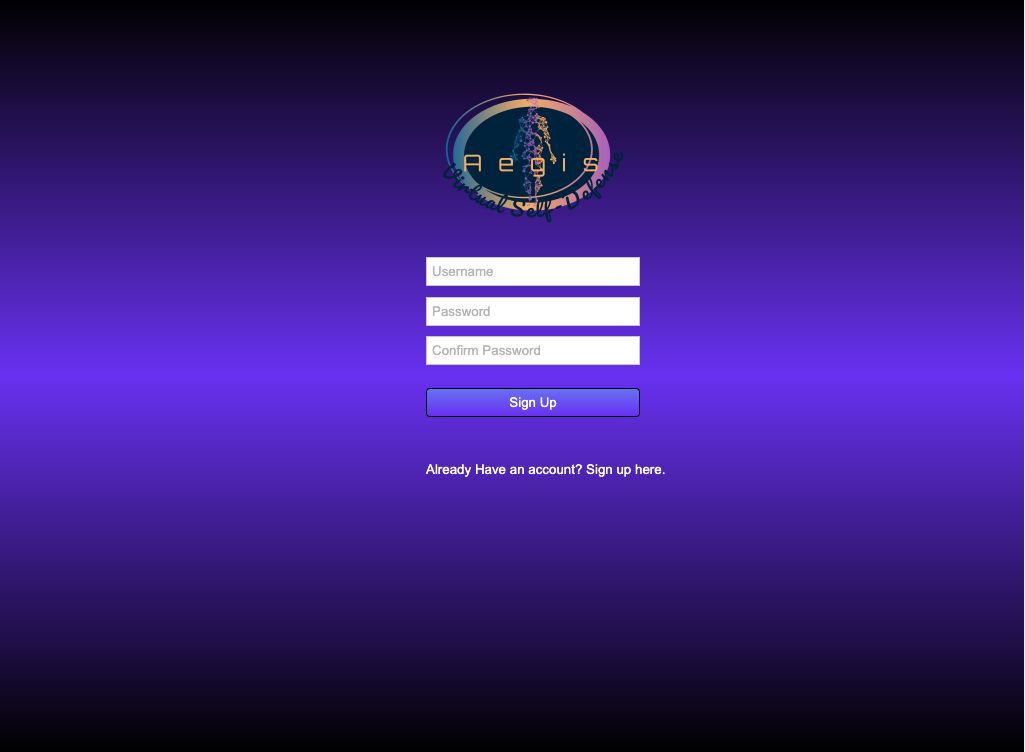
\includegraphics[scale=0.25]{images/Mockups/signup.png} \label{fig:singup} 
  } 
  \quad 
  \subfigure[Login Screen]{% 
    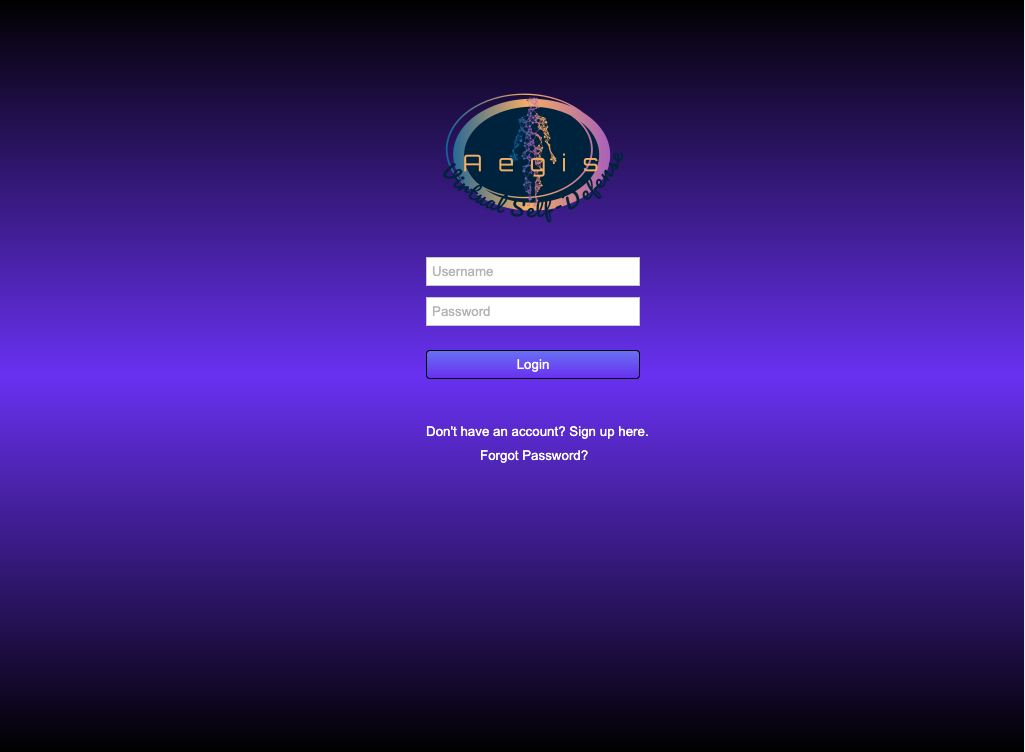
\includegraphics[scale=0.25]{images/Mockups/login.png} \label{fig:login} 
  }
  \quad 
  \subfigure[Change Password Screen]{% 
    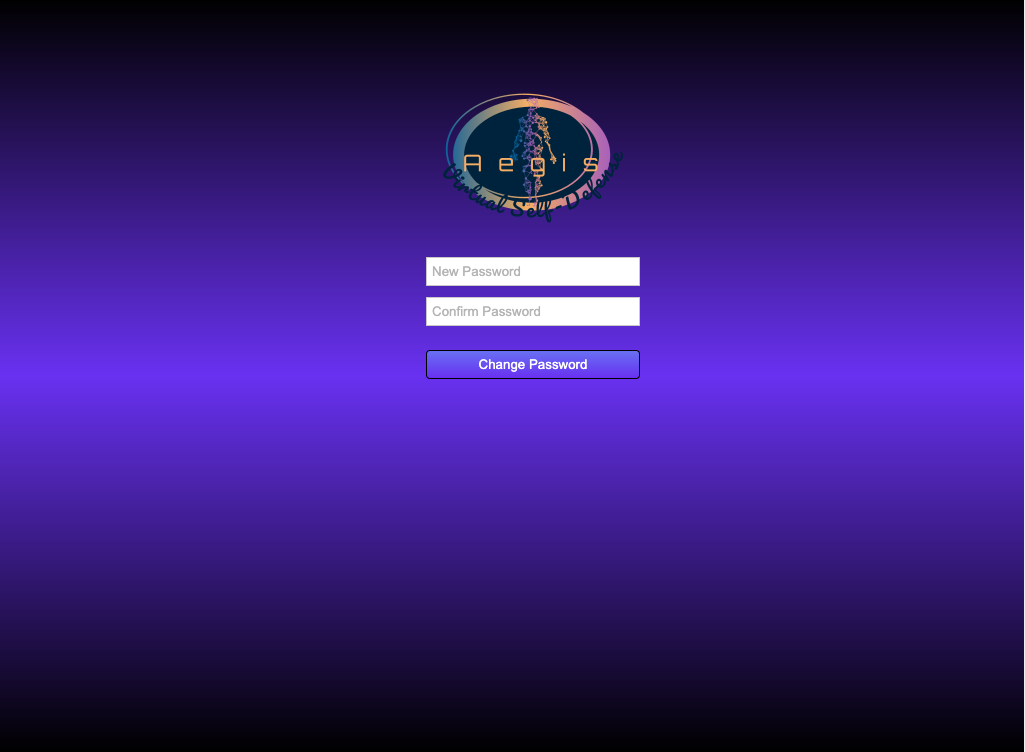
\includegraphics[scale=0.25]{images/Mockups/password.png} \label{fig:password} 
  }
  \caption{Login/Signup Functionality} 
  \centering
  \label{fig:startingScreens}
\end{figure}


Figure \ref{fig:homeTut} shows multiple screens related to home and \textit{Lesson 1} videos. After the user has been granted access to their account, home screen as shown in figure \ref{fig:home} is displayed. This screen gives user the option to choose between \textit{Training} or \textit{Fight} mode. Figure \ref{fig:lesson} shows the screen from where the user can navigate to introductory session of \textit{Lesson 1}, its tutorials and fight session. Screen in figure \ref{fig:intro} will guide the user what they will be learning in \textit{Lesson 1} which will be an animated video. Screen in figure \ref{fig:tutorial} will also display an animated video to the user guiding how a certain technique (specific to that tutorial) should be performed. 

    \begin{figure}
  \subfigure[Home Screen]{% 
    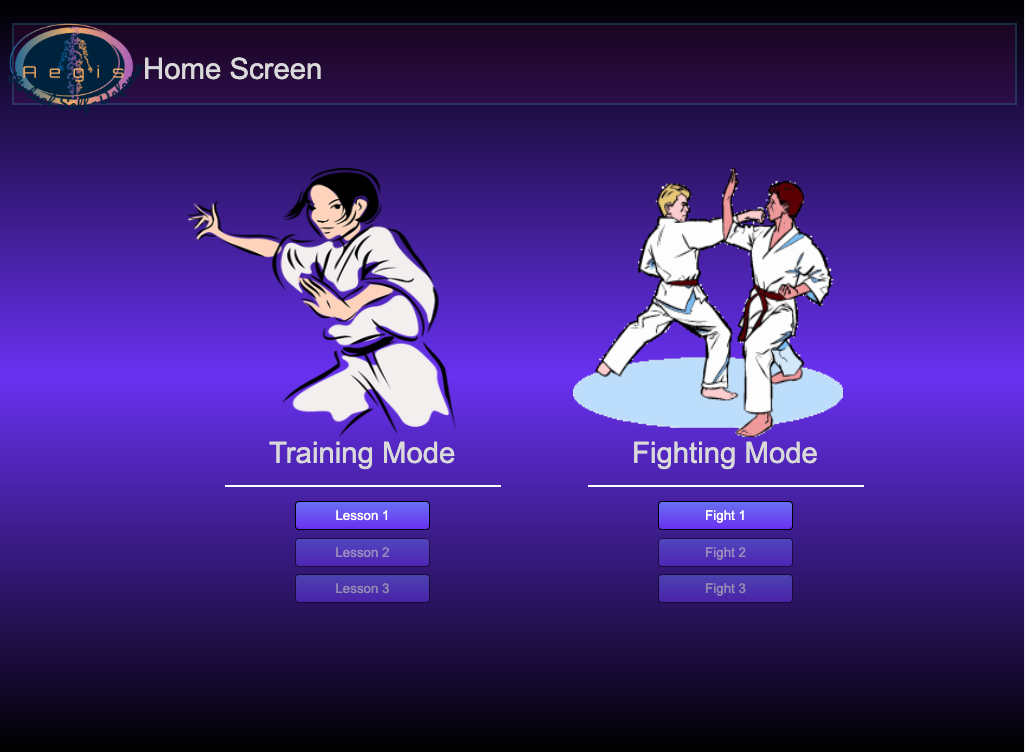
\includegraphics[scale=0.25]{images/Mockups/home.png} \label{fig:home} 
  } 
 \quad 
  \subfigure[Lesson I Screen]{% 
    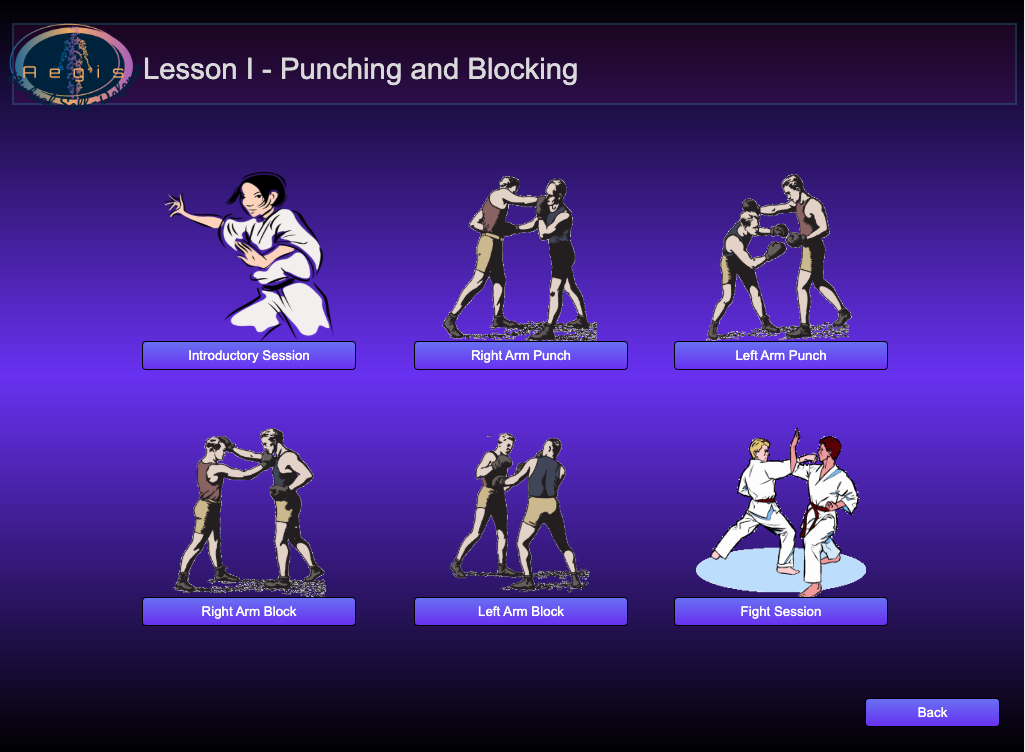
\includegraphics[scale=0.25]{images/Mockups/lesson.png} \label{fig:lesson} 
  } 
  \quad 
  \subfigure[Lesson I: Intro Screen]{% 
    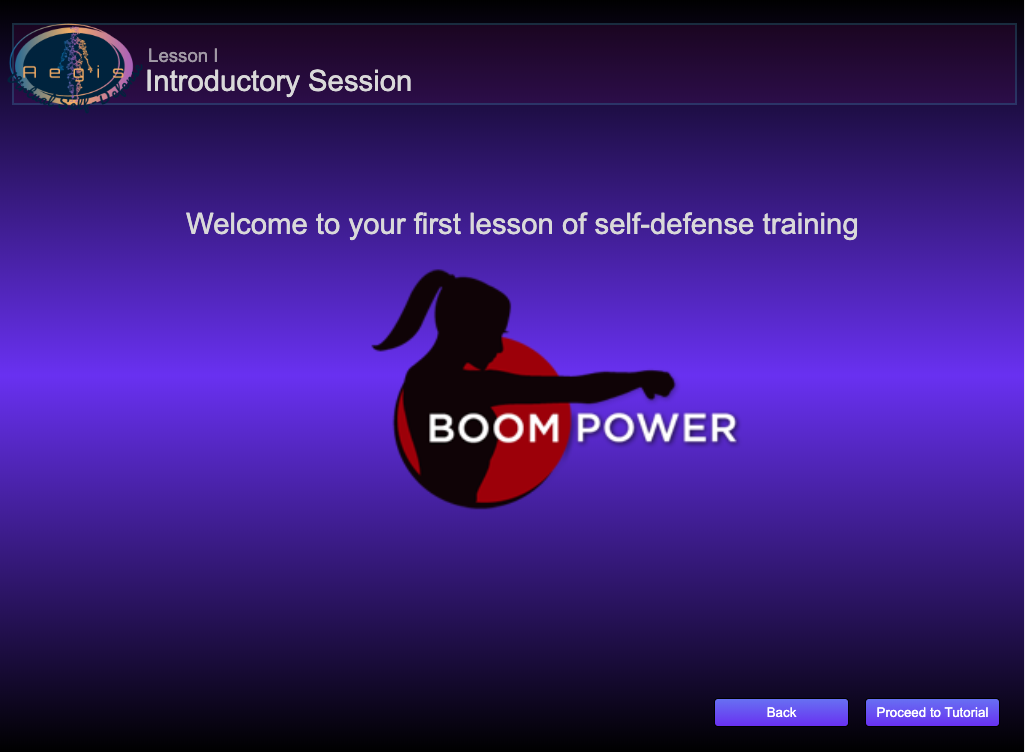
\includegraphics[scale=0.25]{images/Mockups/intro.png} \label{fig:intro} 
  }
  \quad 
  \subfigure[Lesson I: Tutorial I Screen]{% 
    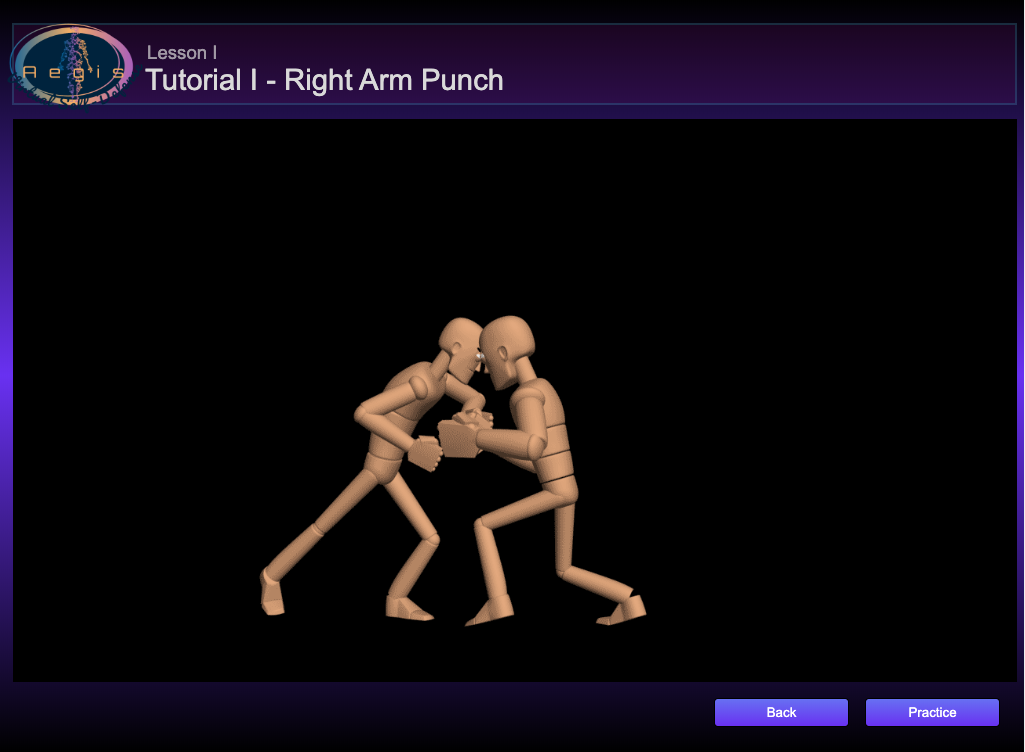
\includegraphics[scale=0.25]{images/Mockups/tutorial.png} \label{fig:tutorial} 
  }
  \caption{Home Screen and Tutorials} 
  \centering
  \label{fig:homeTut}
\end{figure}


Figure \ref{fig:practiceFight} shows screens related to \textit{Practice} and \textit{Fight} sessions. If the user chooses to practice or fight, they will first be asked if they want to do so with a haptic suit as shown in figure \ref{fig:dialogBox}. If the user responds in positive, they will be guided to put their haptic suit on (as shown in figure \ref{fig:haptic}) and will be prompted to calibrate the frequency and amplitude of the haptic signal that they prefer. Figure \ref{fig:practice} and \ref{fig:fight} shows the practice and fight sessions screens. These sessions will start when user clicks the \textit{Start} button. After the session has ended, a feedback report is available on the left.


\begin{figure}
  \subfigure[Haptic Screen]{% 
    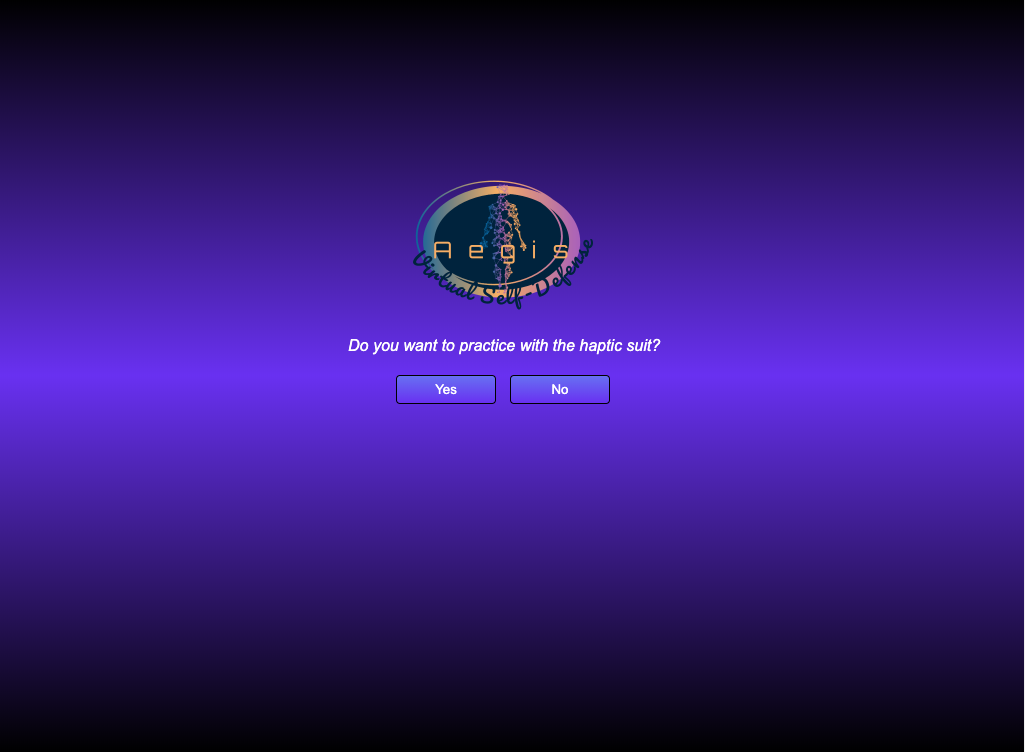
\includegraphics[scale=0.25]{images/Mockups/hapticDialogBox.png} \label{fig:dialogBox} 
  } 
  \quad 
  \subfigure[Haptic Calibration Screen]{% 
    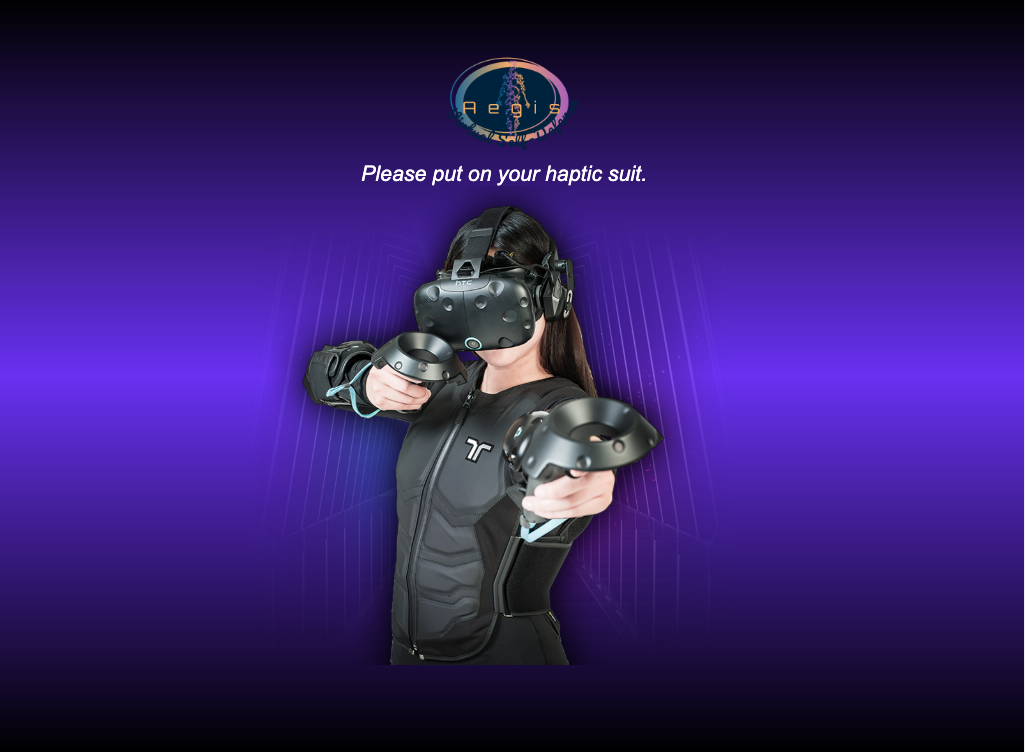
\includegraphics[scale=0.25]{images/Mockups/haptic.png} \label{fig:haptic} 
  } 
  \quad 
  \subfigure[Lesson I Tutorial I: Practice Session Screen]{% 
    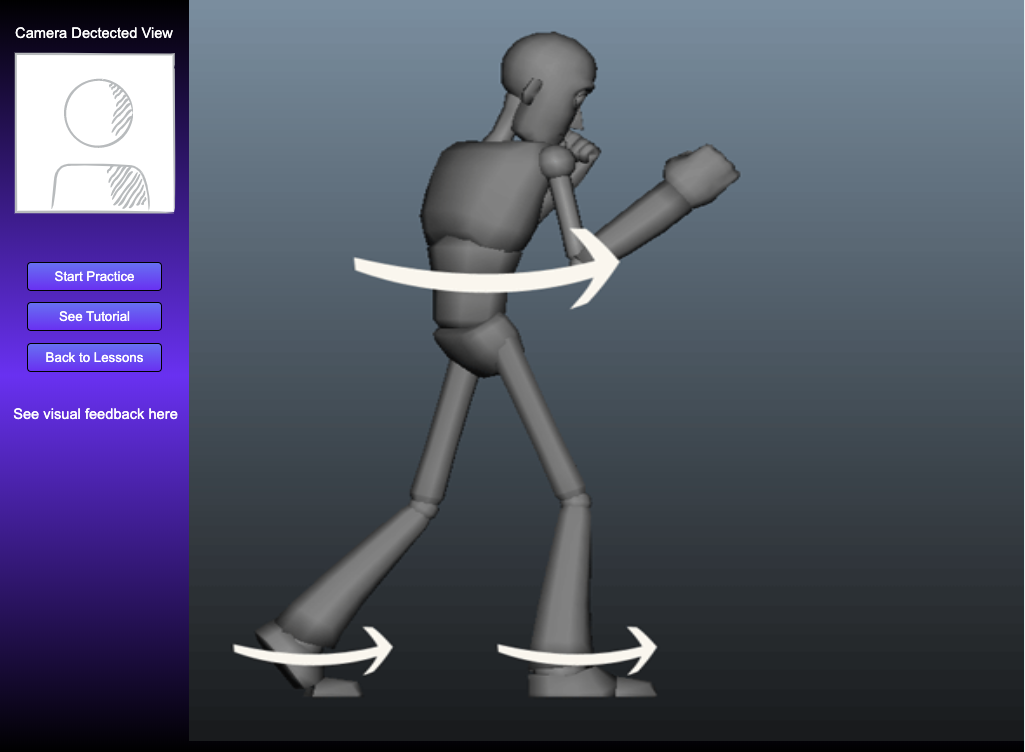
\includegraphics[scale=0.25]{images/Mockups/practice.png} \label{fig:practice} 
  }
  \quad 
  \subfigure[Lesson I: Fight Session Screen]{% 
    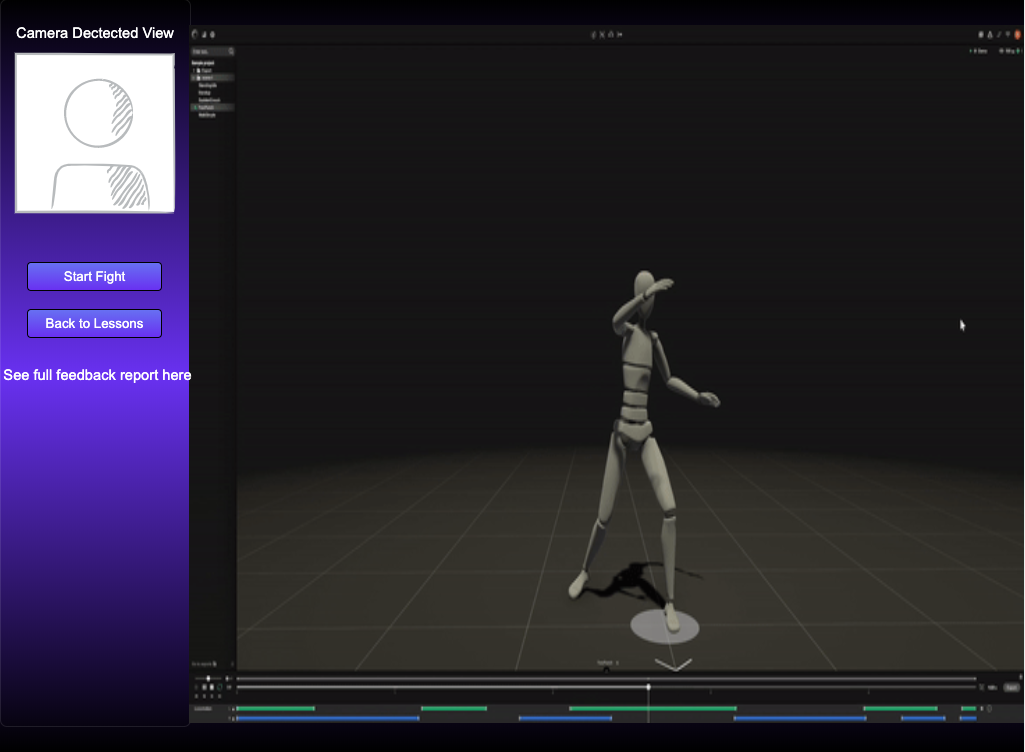
\includegraphics[scale=0.25]{images/Mockups/fight.png} \label{fig:fight} 
  }
  \caption{Practice and Fight Sessions} 
  \centering
  \label{fig:practiceFight}
\end{figure}


\subsection{Hardware/Communication Interfaces}
Since openpose will capture user's movements through a camera, a built-in camera or webcam is required. 
\\
All the hardware will require a connection with power source (9V battery) to power micro-controller, EMS (Electrical Muscle Stimulator) and tens machine.
\\
The Micro-controller will take decisions based on feature and pose vector to on and off some switches which control the tens machine and EMS.
\\
All the communication between hardware and software will be done serially, hence a serial communication cable will be required to transmit and receive data. 

\section{Use Cases}

Figure \ref{fig:usecase} shows the use case diagram of the project, which comprises of the functionalities of the system with respect to the user perspective. 


Following is a short description of the diagram: 


User can login/sign-up into the system and will be granted access after verification of credentials. After that they can either choose \textit{Train Mode} or \textit{Fight Mode}. The \textit{Train Mode} further includes tutorials and practice sessions. Both fight sessions and practice sessions provide user feedback indicating how well the user performed and how he can improve it. In addition to feedback, fight session also suggest tutorials based on areas the system thinks user has performed poorly. In case a user is fighting or practicing with haptics, they first need to calibrate the frequency and amplitude of the signal at which they are most comfortable.


\begin{figure}
    \centering
    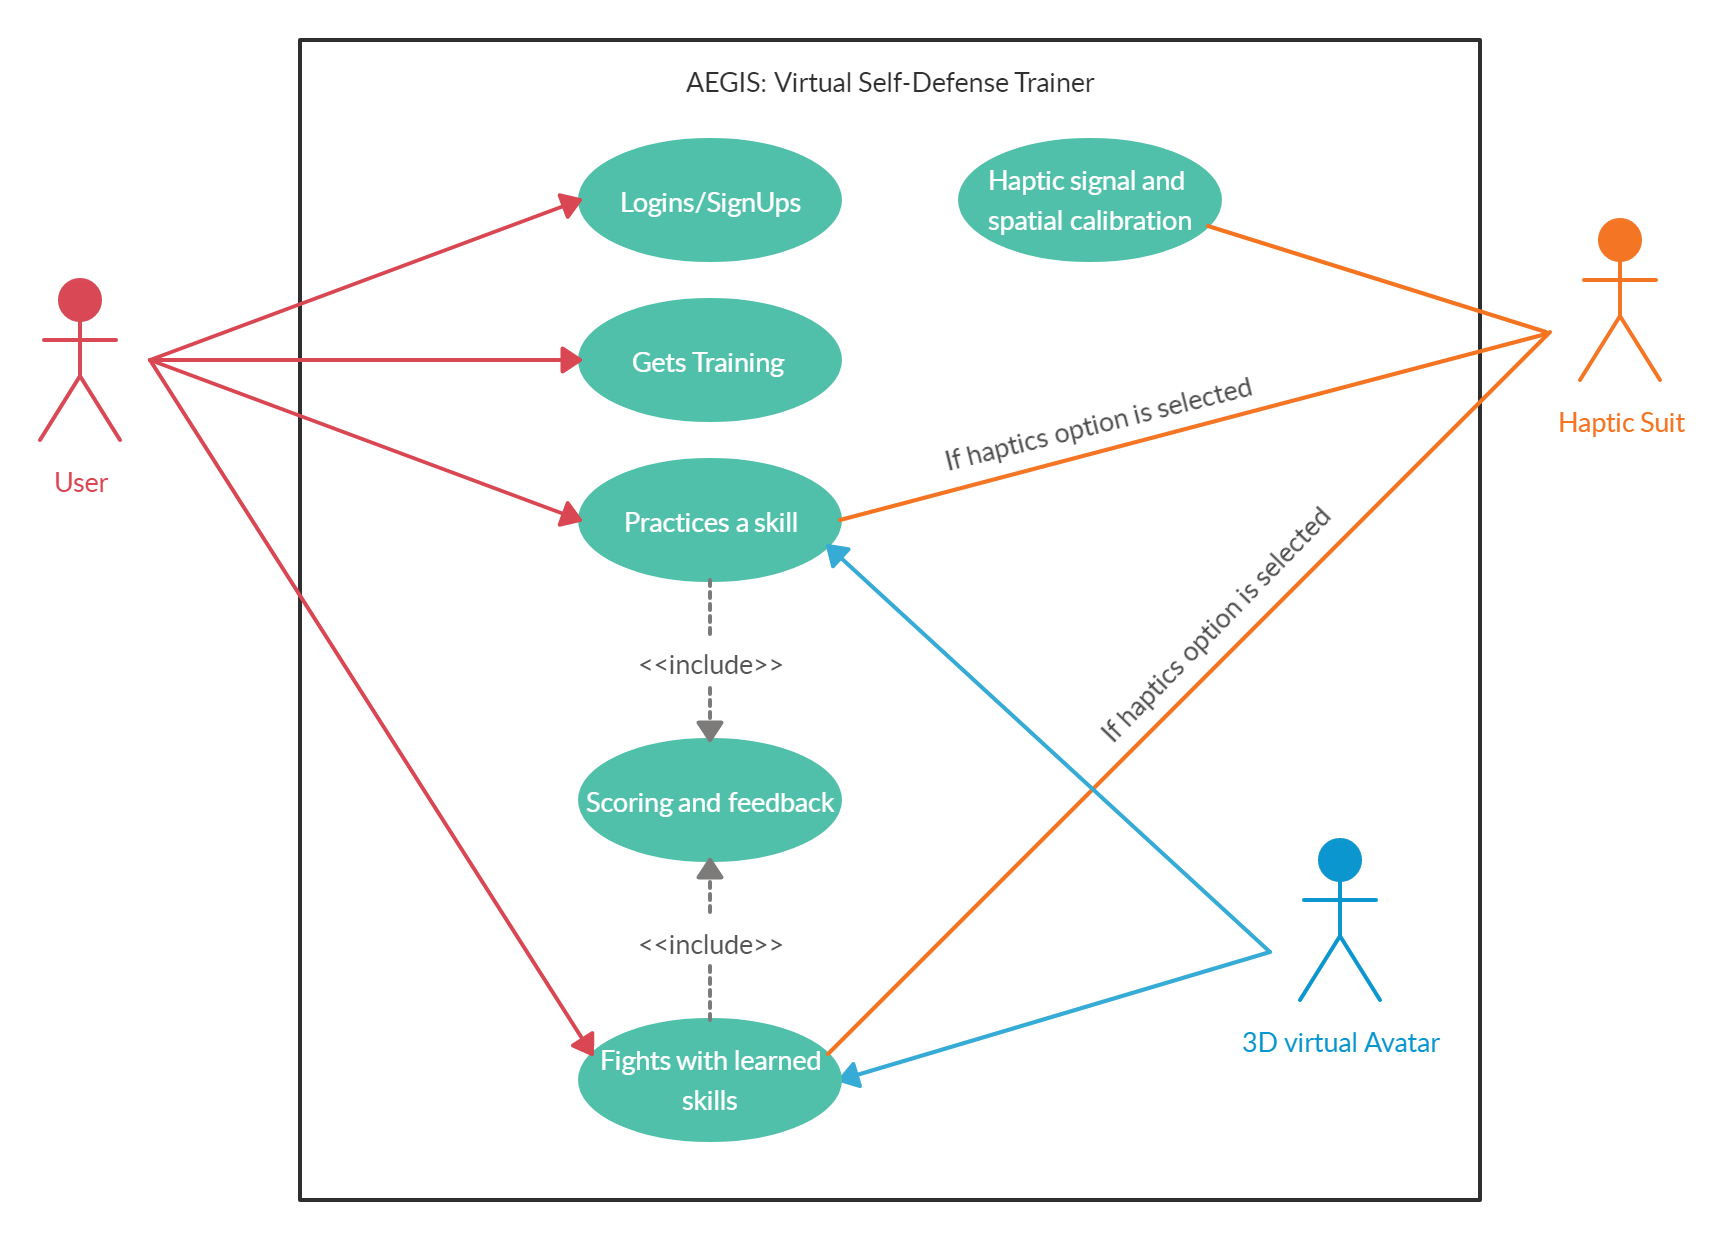
\includegraphics[scale=0.28]{images/UseCaseDiagram.png}
    \caption{Use Case Diagram}
    \label{fig:usecase}
\end{figure}


\section{Datasets}

There are no external datasets being used in this project. We have recorded our own videos for tutorials, and videos that serves as benchmark for pose evaluation and will be used in similarity comparison for pose classification. For validation of the system, we have created three classes of videos, having good, satisfactory and poor performance of the punch-block sequence.

\section{System Diagram}

\begin{figure}
    \centering
    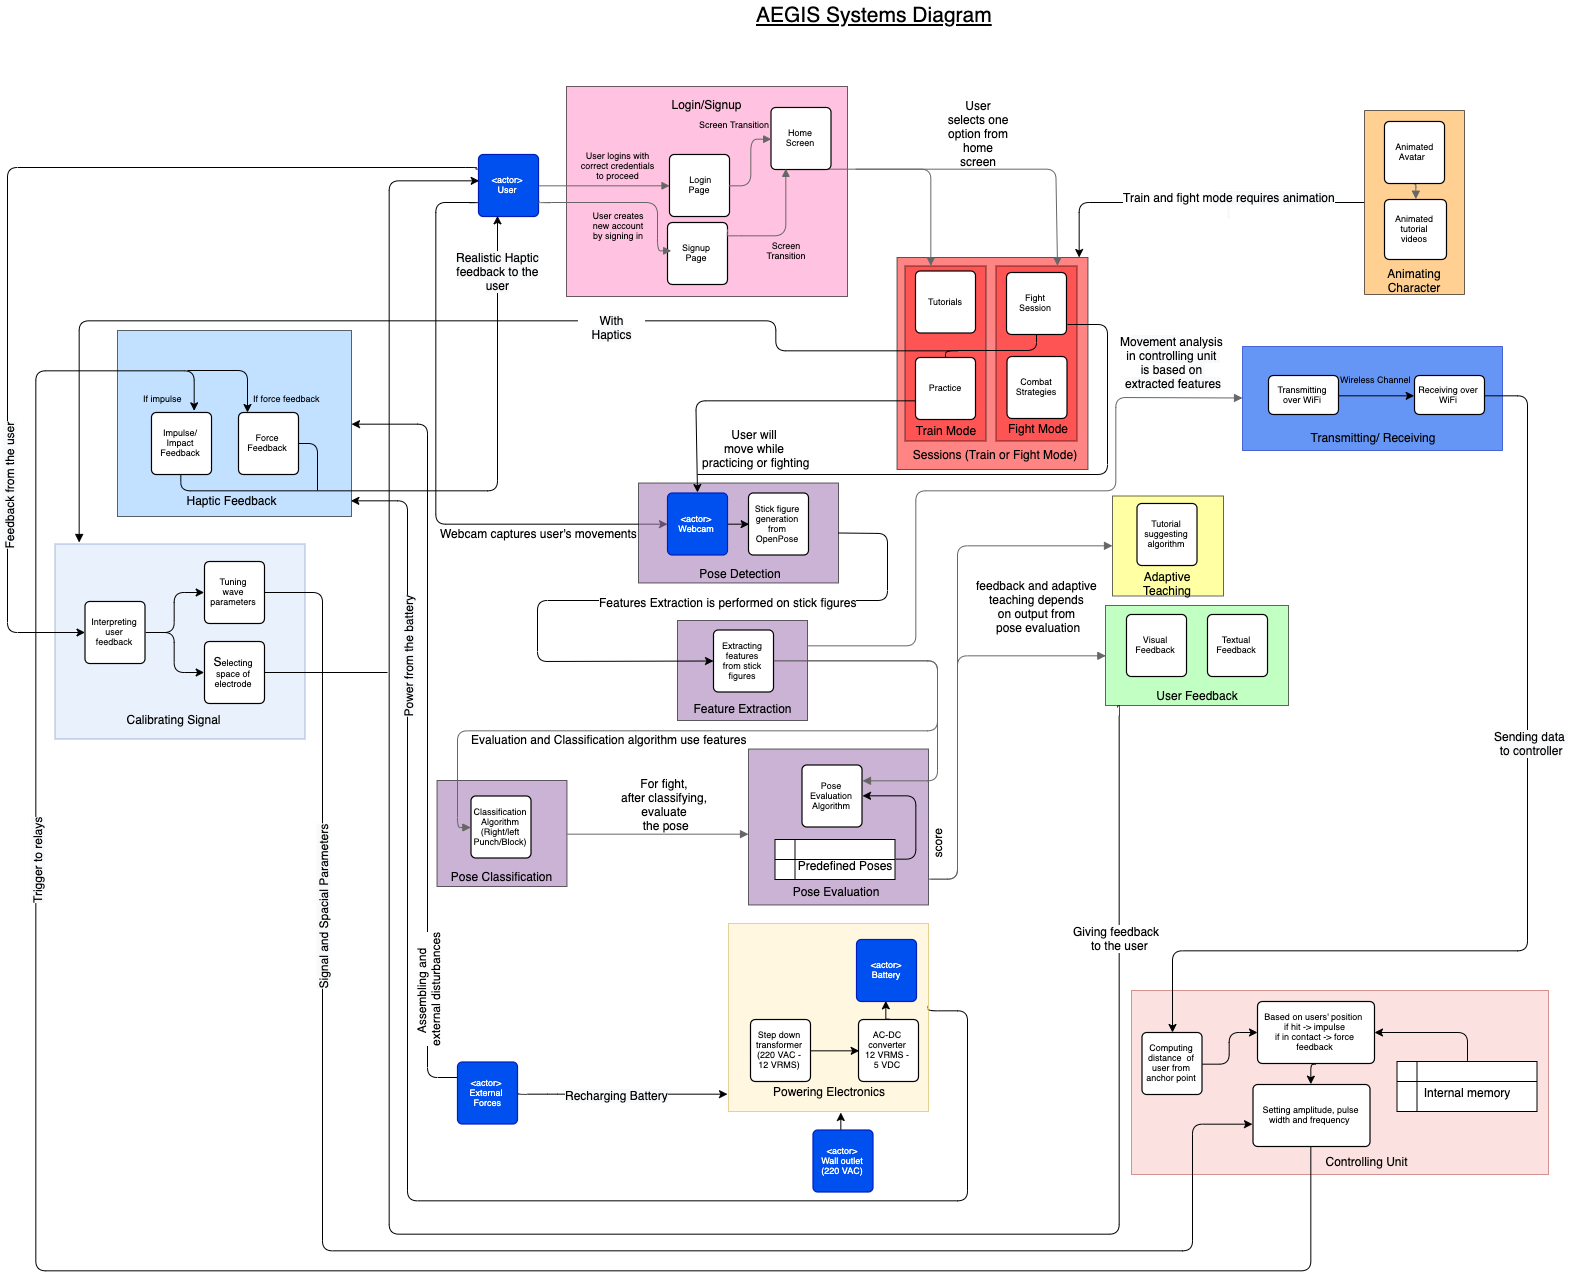
\includegraphics[scale=0.4]{images/SystemDiagram.png}
    \caption{System Diagram}
    \label{fig:systemDiagram}
\end{figure}

\clearpage

Figure \ref{fig:systemDiagram} shows the system diagram of our system which gives a high-level view of the different components of our system and the interactions between them. Each actor, component and the particular tools/technologies/libraries used to build it are described below.

\subsection{User}
User interacts with a few sub-systems in the main system. First of all, the user completes the sign-up or log-in step. This information is stored in the system's database and the process continues to either a \textit{Train Mode} or \textit{Fight Mode}. Hence, user outputs a selected mode, and in addition to that the user also outputs feedback to the calibration protocol if they choose to interact with haptics. The inputs to the user will be the haptic feedback, user feedback and visual display based on which it will interact with the system.

\subsection{Login/SignUp Module}
The input to this module are the user credentials (ID and password), and upon successful login/signup, the user can output a selection between train or fight mode.

\subsection{Animating Character Module}
This block is required to animate the avatar for the practice and fight session. This block will also animate user's body parts which will be in the view of the camera (like hands). 

\subsection{Sessions Module}
There are two modes that the user will select, either fight or train mode. Train mode is further divided into tutorials and practice sessions, while fight mode contains fight sessions along with avatar's combat strategies. Both the modes require animations from the animation module. 

\subsection{Calibrating Signal Module}
Before these sessions, if the user selects \textit{with haptics} then the haptics component needs to be calibrated. The calibration scheme consists of an automatic protocol that takes in user’s feedback as input to calibrate the parameters of wave (pulse width, frequency and amplitude of the EMS waves). These will be sent to the controlling unit and the controlling unit will tune in the parameters accordingly. Based on this, the output of the haptics will be modified, and the user will rate these modified sensations. This loop will continue until the sensation lies perfectly according to user's comfort. 

\subsection{Controlling Unit Module}
This block is comprised of primarily Arduino or any IoT platform. This will take in inputs over WiFi/cable from the Feature Extraction Module. Based on the feature vector, it will send in triggers and the parameters to the haptic block. This will make decisions as to which haptic signal to activate (impulse or force feedback). Based on distance of the user from the avatar it will activate the relays by comparing the distances with the pre-stored data and conditions in the memory. This also takes part in the calibration scheme where it gets information from the protocol and sets parameters accordingly.

\subsection{Haptic Feedback Module}
This block has two types of outputs, either a force feedback or an impulse feedback. The information about the wave parameters and when to activate comes directly from the Control Unit module. The output is directly exposed to the user. It makes the user feel the virtual environment.

\subsection{Transmission/Receiving Block}
This block gets the output from the feature extraction module and sends the feature vector to the control unit which makes decisions as described in Controlling Unit Module.

\subsection{Pose Detection Module}
This takes images from the webcam as inputs and outputs a series of time-dependent raw pose vectors in a csv file. This will be sent to the feature extraction module.

\subsection{Feature Extraction}
This module takes a series of time-dependent raw pose vectors in form of csv files as input and outputs features like velocity, acceleration, kinetic energy etc. This feature vector/tensor will be sent to the control unit and also to the pose classification block in the case of a fight session, before finally sending it to the pose evaluation module.

\subsection{Pose Evaluation Module}
This block gets input from the feature extraction block. This input feature vector is compared with the benchmark feature vector of predefined pose. Based on this comparison the score is given. The score is then sent to adaptive teaching block and the user feedback block.

\subsection{User Feedback Module}
This block gives feedback in natural language on based on the numerical score. The feedback will be sent to the display.

\subsection{Adaptive Teaching}
This component suggests the next tutorial based on the current performance score. The input is the score from pose evaluation and the outputs are the suggested tutorials that the user should practice more. 

\subsection{Powering Electronics}
This block recharges the battery and powers the entire circuitry including the haptic suit, the controlling unit, and the desktop (PC). 

\subsection{External Forces}
These are forces used for assembling in order to put the suit together. These external forces are at play when the user interacts with it whilst wearing the suit and recharging its battery (plug forces).






\chapter{Software Design Specification\\ (SDS)}
\label{chap:sds}
This chapter provides important artifacts related to design of our project.

\section{Software Design}

This section presents the UML class diagram and gives a brief description of each class in our system. Attributes and methods of each class and relationship among classes are clearly presented.

Figure \ref{fig:UML_Unity} describes the UML of the software made in Unity 3D. The \texttt{SoftwareController} acts as the main controller of the entire engine and is also responsible for \texttt{GET} and \texttt{POST} requests to the firebase database, whereas the \texttt{VideoController} and \texttt{SliderController} are used for viewing video and gives its control options. The rest of the controllers are Screen Controllers which are child objects to \texttt{Screen} type gameobjects made in Unity. These controller of each screen is defined according to the activity involved in that interface. 

Figure \ref{fig:UML_PoseEvaluation} describes the UML of the pose evaluation module. \texttt{Features} class is responsible for extracting the features out of \texttt{PoseData} objects constructed through \texttt{.csv} files generated by \texttt{PoseEstimator} class. The \texttt{Features} class uses \texttt{SmoothingFilter} for data smoothing and filtering and for getting derivatives. These extracted features are used by \texttt{PoseEvaluator} class which temporaly aligns the necessary features and generates feedback. The feedback is generated on the basis of individual feature scores provided by \texttt{PoseEvaluator}. 

\begin{figure}
  \centering
  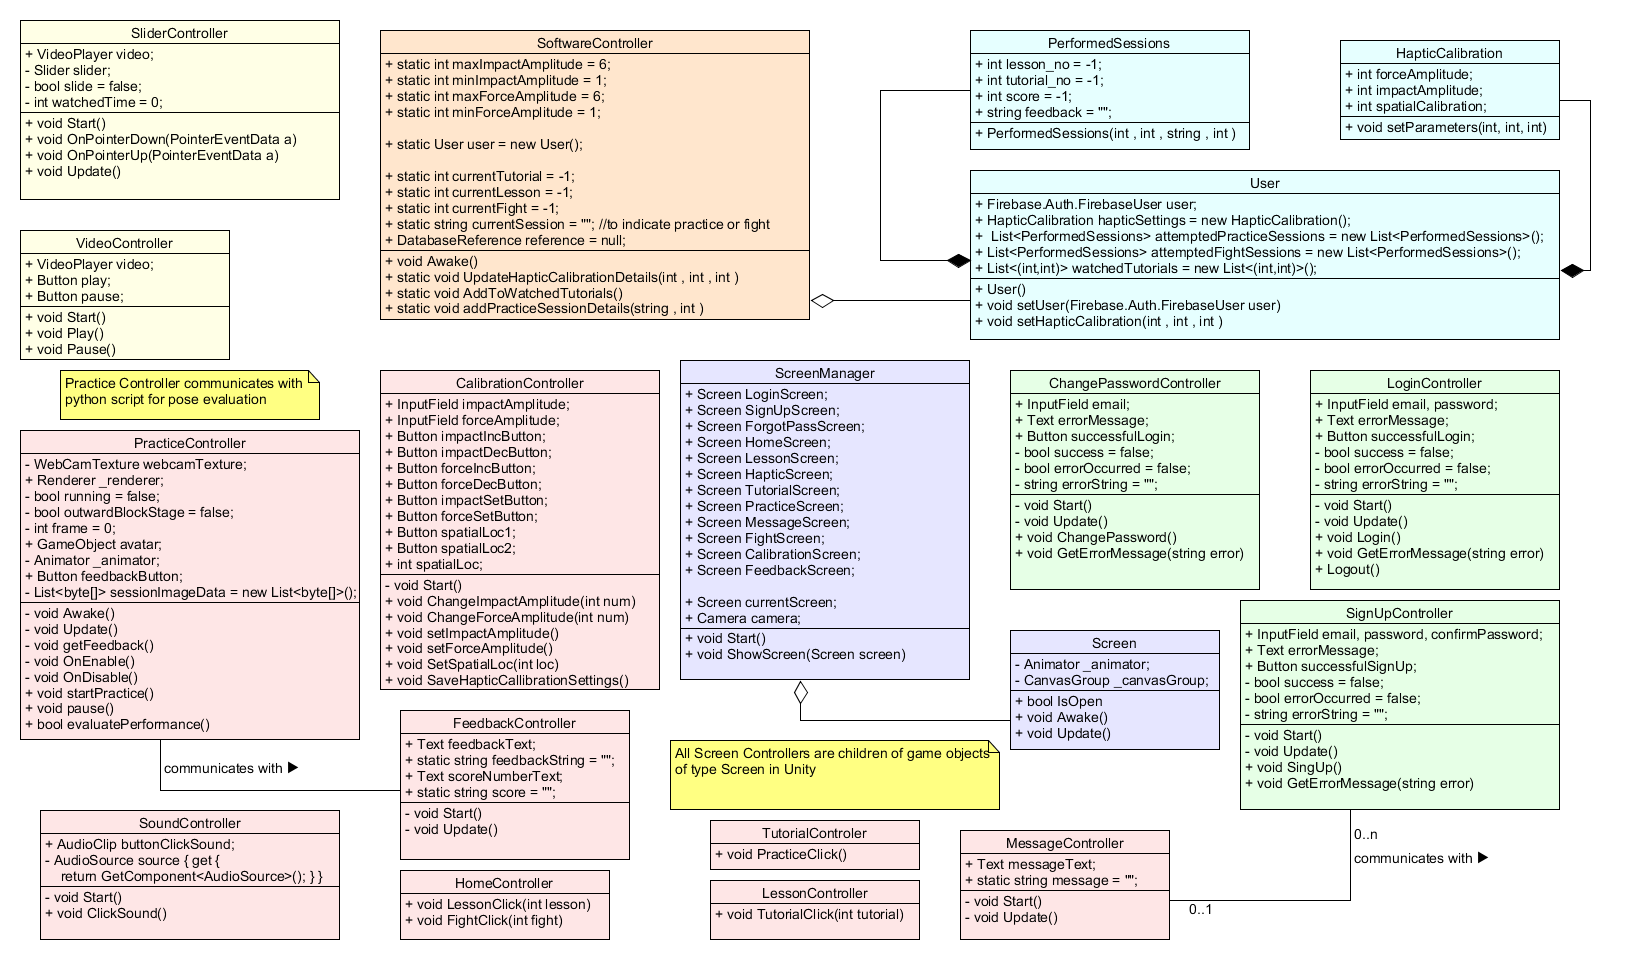
\includegraphics[scale=0.3]{images/UML - Unity Software.png}
  \caption{UML of the Unity Software}
  \label{fig:UML_Unity}
\end{figure}

\begin{figure}
  \centering
  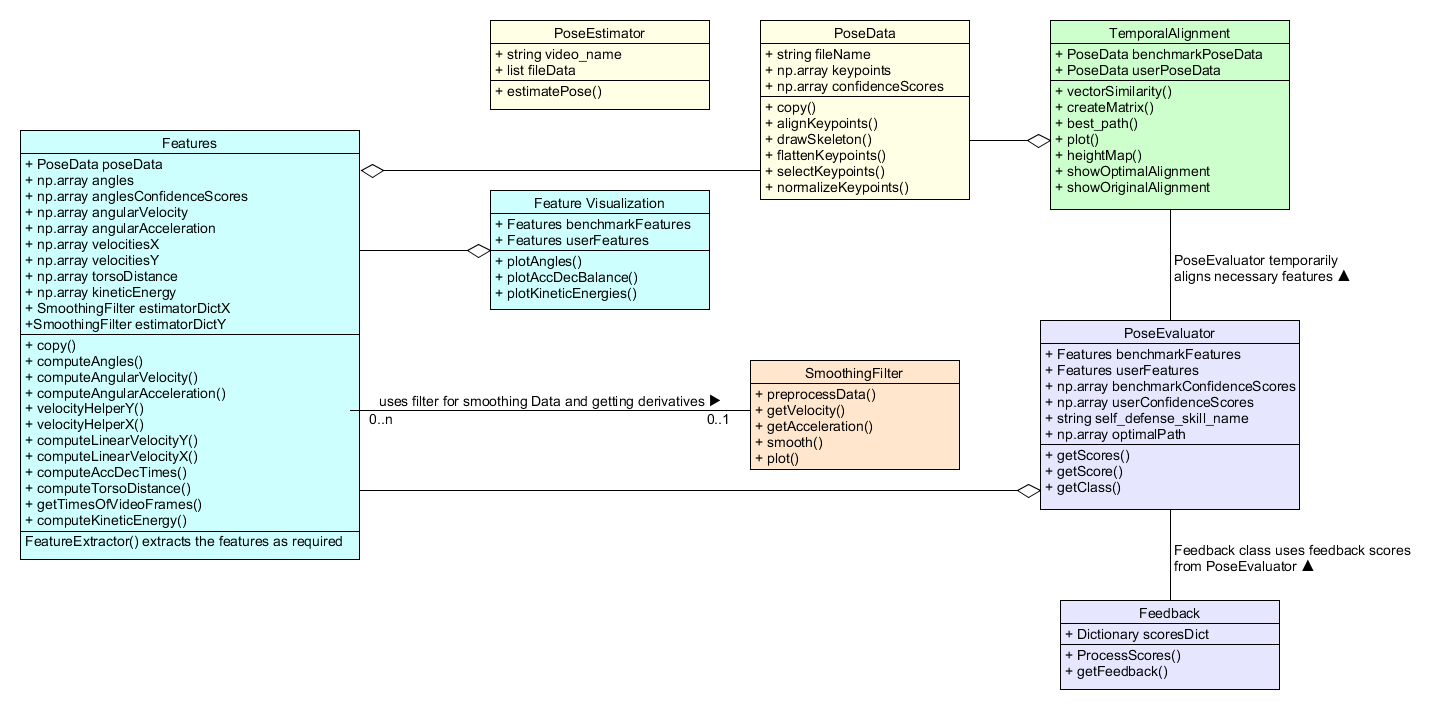
\includegraphics[scale=0.34]{images/UML - Pose Evaluation Module.png}
  \caption{UML of the Pose Evaluation Module}
  \label{fig:UML_PoseEvaluation}
\end{figure}


% Your report will contain ONE of the following 2 sections.

\section{Data Design}

This section presents the structure of our database that caters to persistent data storage in our project. The structure is shown in figure \ref{fig:RelationalDatabase} is a normalized data model for relational databases. It clearly shows entities, attributes, relationships with their cardinalities, and primary and foreign keys. We have used DB designer to build our data model.


Each user will have a username and password. We need to save the so far progress of the user, for example, how many tutorials they have watched, how many practice and fight sessions they attempted and what score and feedback they received in those and what settings of haptics they calibrated according to their comfort level. In addition to user based data, we also need to store which video and animated tutorial to display in which tutorial and practice session, because these tutorial and practice screens have the same GUI, only their animation changes. If a user has attempted a fight session, we also need to store what tutorials were suggested to them by the system, in case the user feels the need to go back to them. For pose classification and evaluation, we also need to store benchmark videos of different self-defense moves along with their extracted key-points. Their extracted features are stored in a different table because many different features can be extracted from each move. 

\begin{figure}
    \centering
    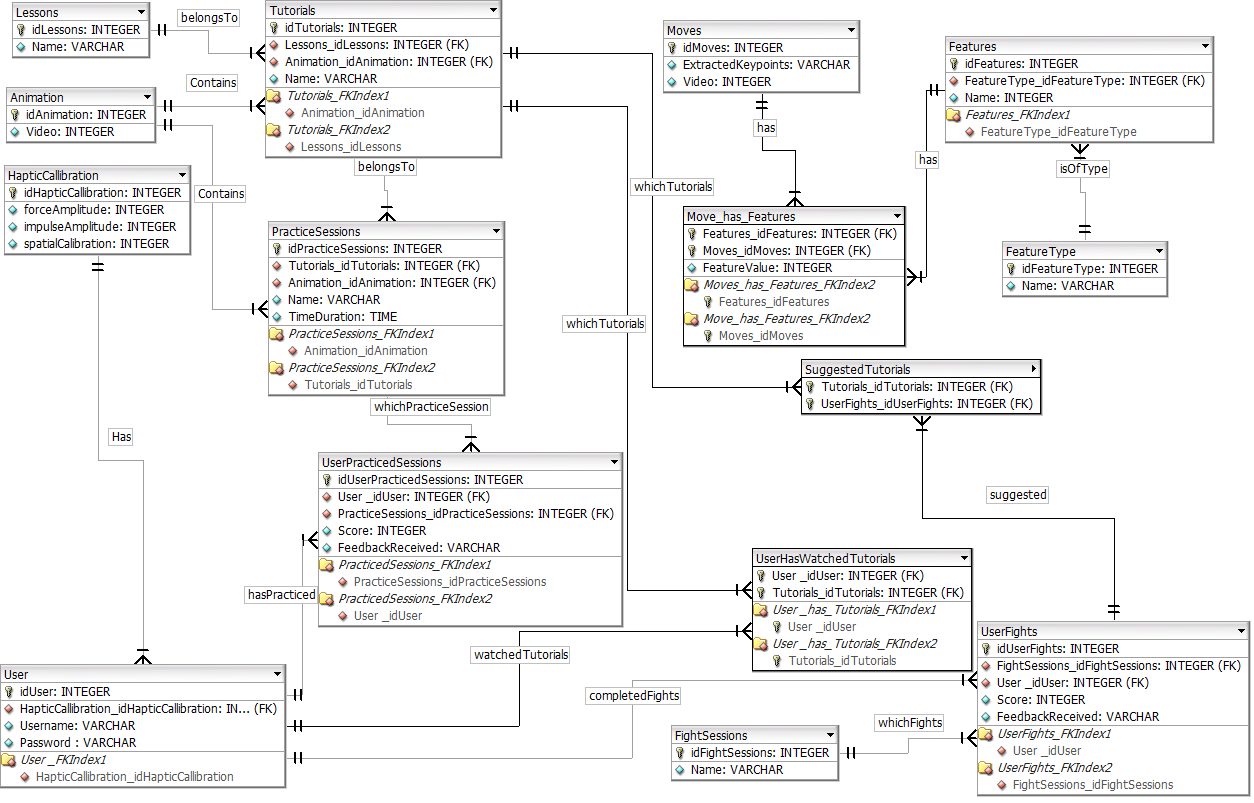
\includegraphics[scale=0.38]{images/databaseDesign.png}
    \caption{Relational Database}
    \label{fig:RelationalDatabase}
\end{figure}


\section{User Interface Design}
The user interface is built on unity game engine. 
Figure \ref{fig:credentials} shows the user interface for handling user authentication and updating credentials. The authentication is done via using Firebase Authentication SDK for Unity by manually integrating their authentication methods into the unity software. It is an email and password based authentication which authenticate users with their email addresses and passwords. The Firebase Authentication SDK provides methods to create and manage users that use their email addresses and passwords to sign in, and it also handles sending password reset emails. 

\begin{figure}
    \centering
    \subfigure[Login Screen]{% 
      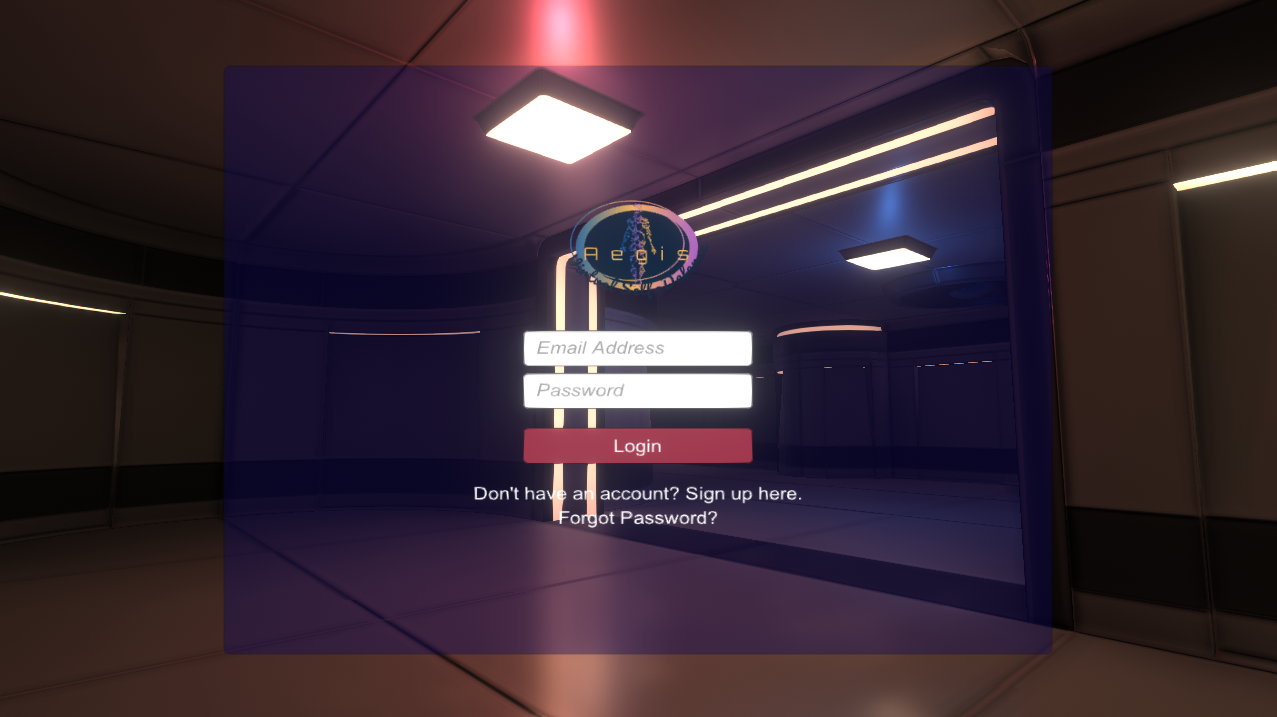
\includegraphics[scale=0.31]{images/screens/login.png} \label{fig:loginUnity} 
    } 
   \quad 
    \subfigure[SignUp Screen]{% 
     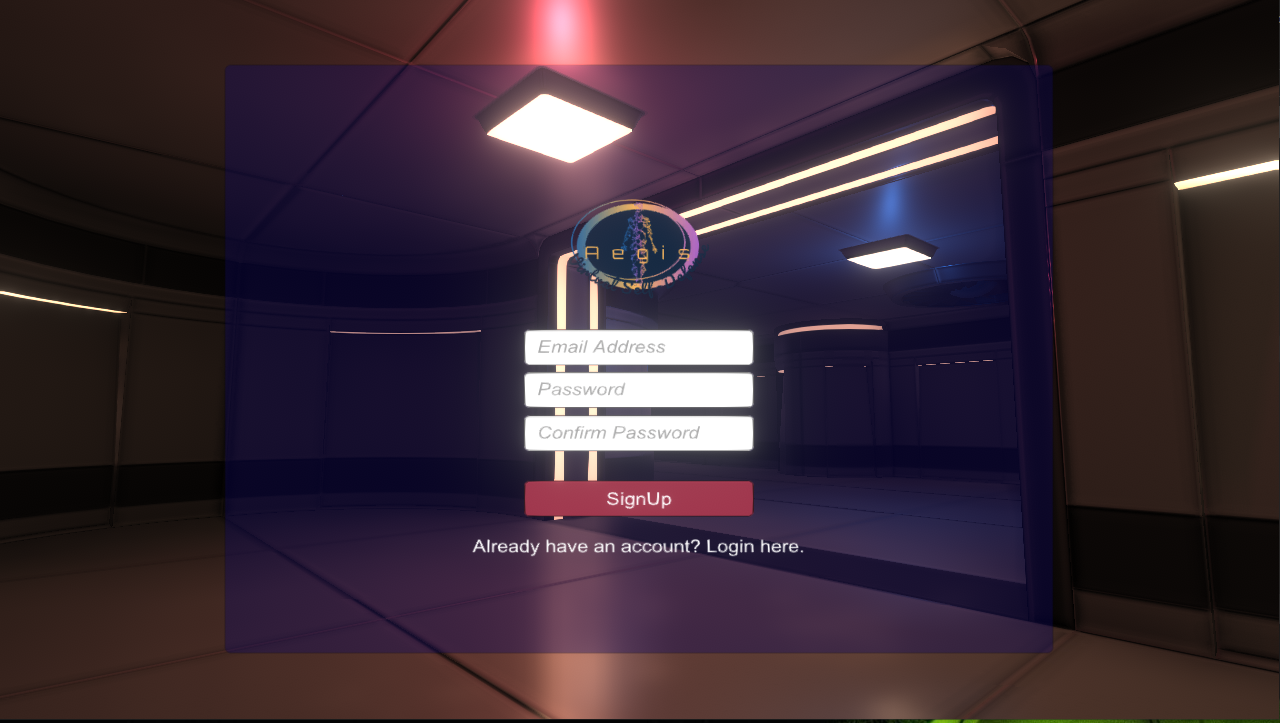
\includegraphics[scale=0.31]{images/screens/signUp.png}     \label{fig:signUp} 
    } \\
    \quad 
    \subfigure[Forgot Password Screen]{% 
      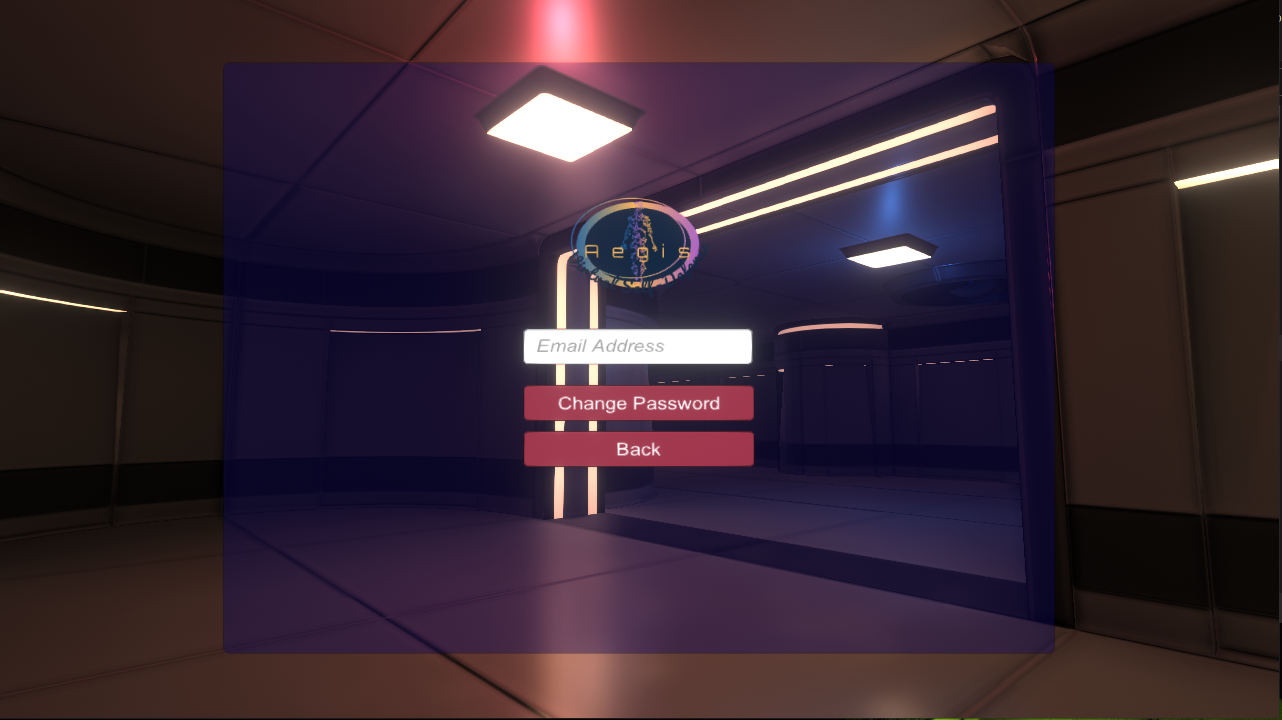
\includegraphics[scale=0.31]{images/screens/forgotPassword.png} 
      \label{fig:forgotPassword} 
    }
    \caption{User Interface for Authentication} 
    \label{fig:credentials}
\end{figure}

Figure \ref{fig:homeScreen} shows the main menu (home screen) display when the user is granted access to the system. The home screen gives the user the option to either select training mode or fighting mode. 

\begin{figure}
    \centering
    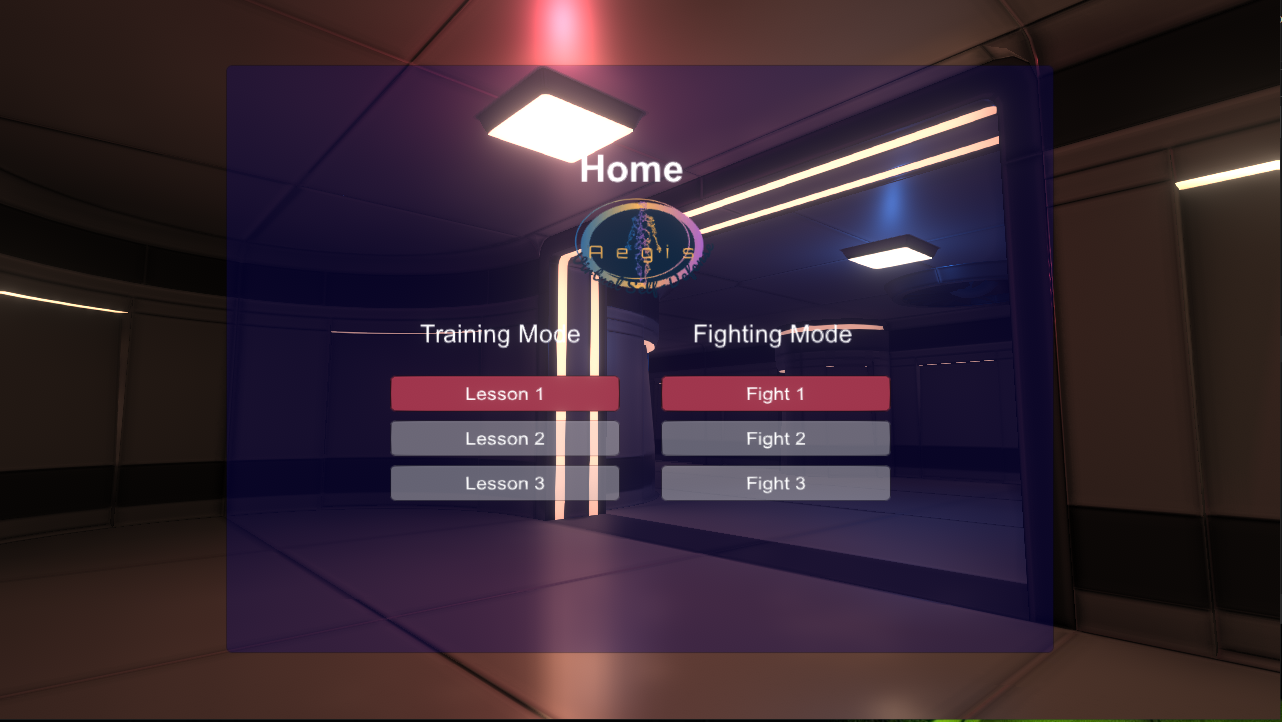
\includegraphics[scale=.5]{images/screens/home.png}
    \caption{User Interface for Main Menu}
    \label{fig:homeScreen}
\end{figure}

Since our system is modular, it allows the liberty of practising without the haptic suit. However, without it, the software won't be able to give full human trainer like realistic experience. This option solely exists to cater to those not comfortable in wearing the haptic suit. Therefore, before proceeding to any practice or fight session, the system prompts the user to select their preference as shown in figure \ref{fig:hapticPrompt}. In case the user chooses to practice with the haptic suit, the software requires haptic calibration prior to proceeding any further as shown in figure \ref{fig:hapticCallibration}. The user must calibrate amplitude as well as the spatial position of electrodes as anatomical variations are the biggest limitation of EMS. Once calibrated, these settings will be stored in the Firebase Database. 

\begin{figure}
    \centering
    \subfigure[Haptic Prompt Screen]{% 
      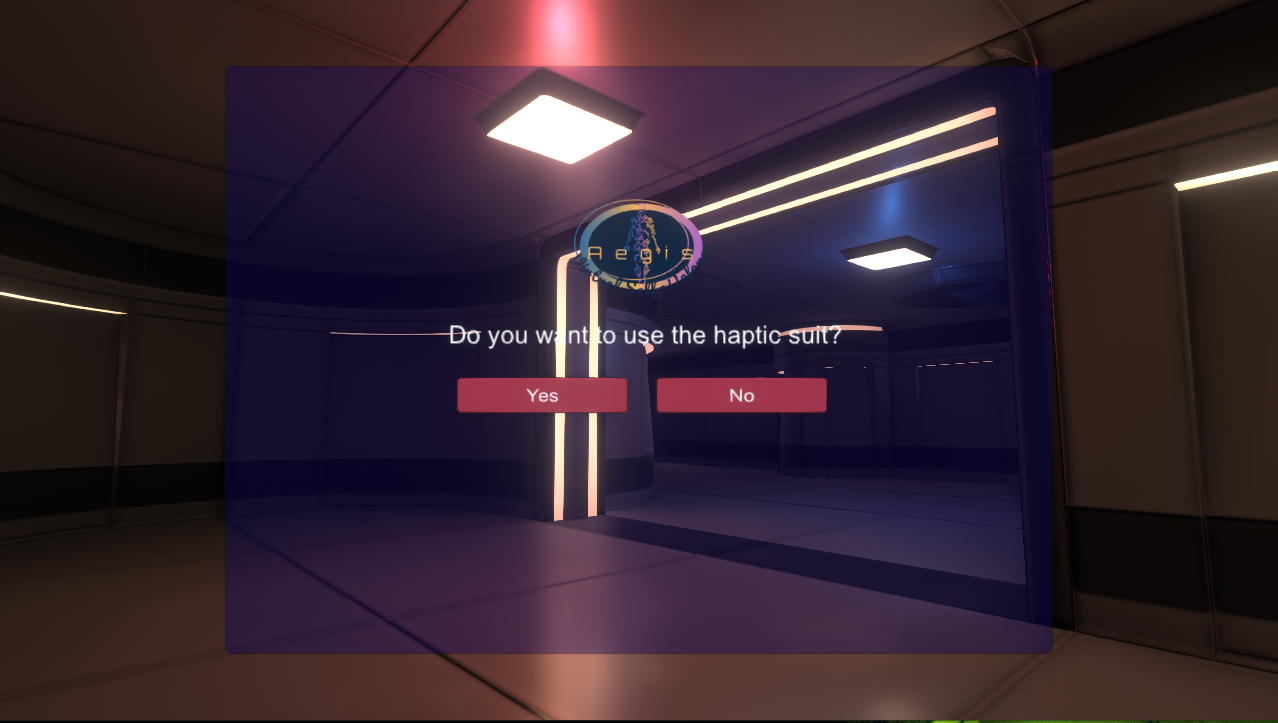
\includegraphics[scale=0.31]{images/screens/hapticPrompt.png} 
      \label{fig:hapticPrompt} 
    } 
   \quad 
    \subfigure[Haptic Callibration Screen]{% 
     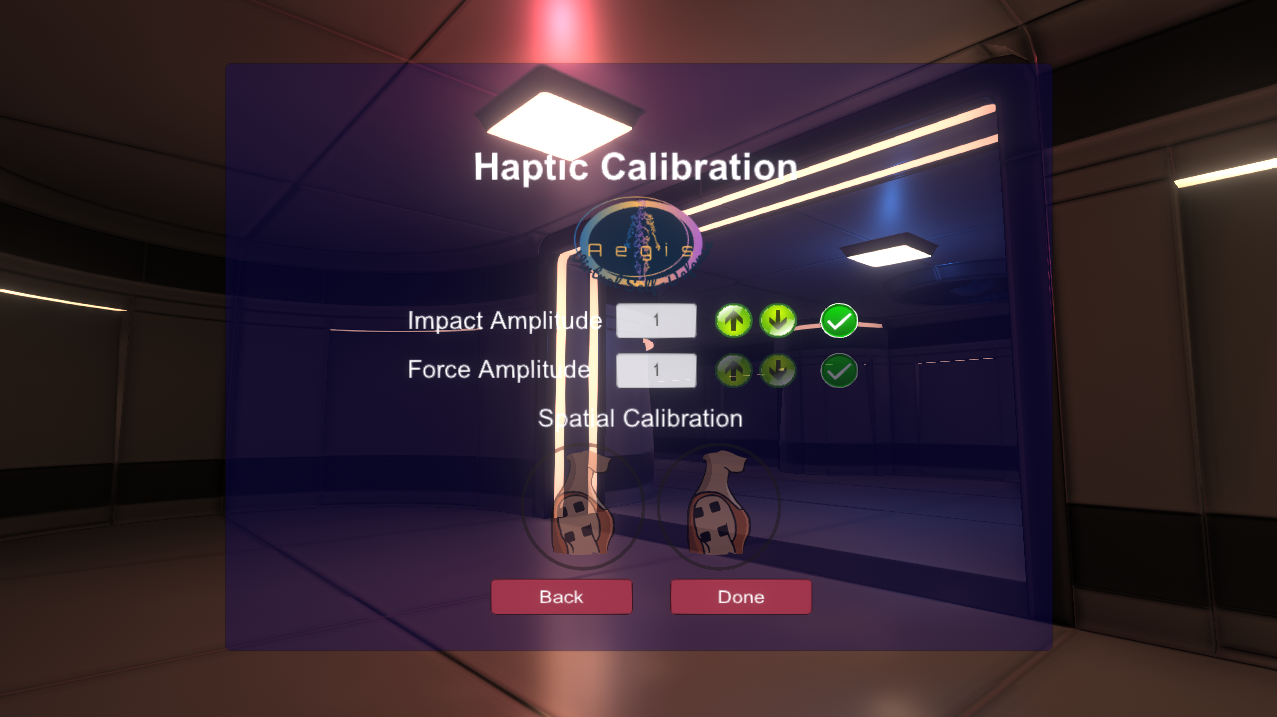
\includegraphics[scale=0.31]{images/screens/hapticCallibration.png}     
     \label{fig:hapticCallibration} 
    }
    \caption{User Interface for Selecting and Calibrating Haptics} 
    \label{fig:hapticScreen}
\end{figure}

Figure \ref{fig:tutorials} shows the user interface for lessons and tutorials. The training mode contains lessons, tutorials and practice sessions, whereas the fighting mode contain fight sessions of corresponding lessons. Each tutorial teaches a specific skill through a video as shown in figure \ref{fig:tutorialUnity}. 

\begin{figure}
    \centering
    \subfigure[Lessons Screen]{% 
      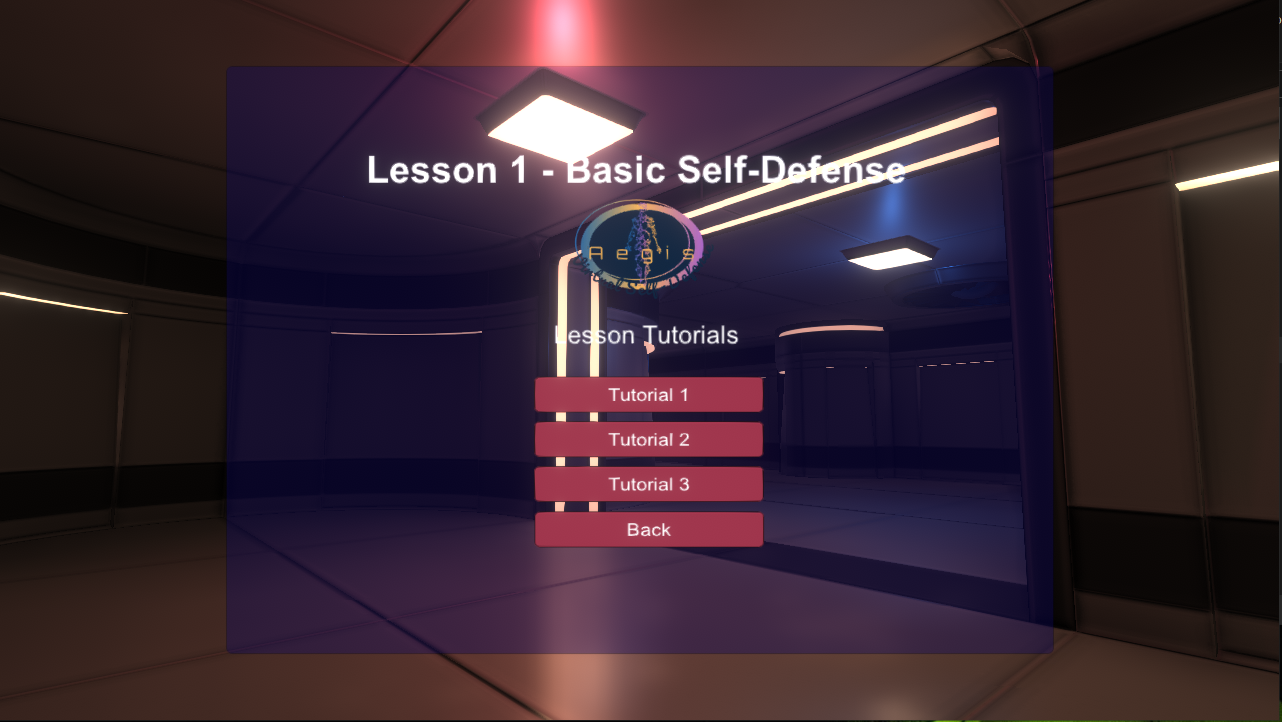
\includegraphics[scale=0.3]{images/screens/lesson.png} \label{fig:lessonUnity} 
    } 
    \quad 
    \subfigure[Tutorial Screen]{% 
      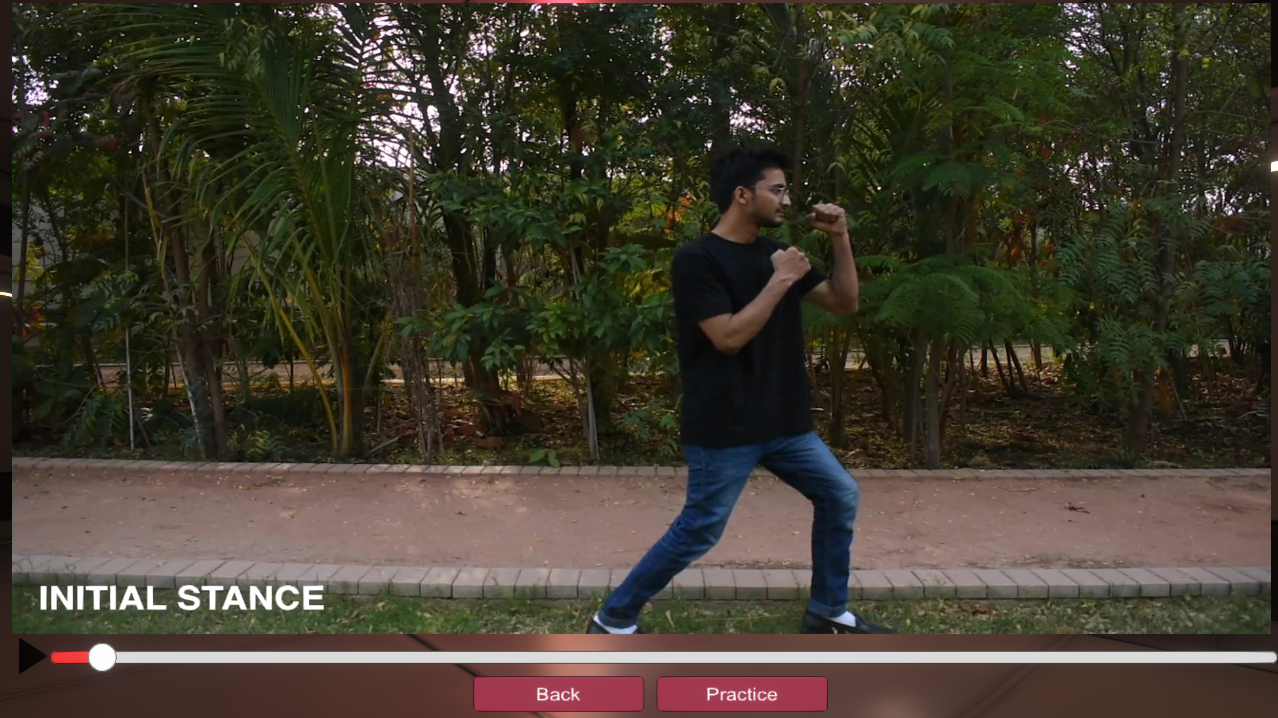
\includegraphics[scale=0.3]{images/screens/tutorial.png} \label{fig:tutorialUnity} 
    }
    \caption{User Interface for Lessons and Tutorials} 
    \label{fig:tutorials}
\end{figure}

For practice and fight sessions, an animated avatar attacks the user, requiring them to attack the avatar back in defense based on the skills taught. These practice and fight sessions are started when a button click event is triggered by the user, which then signals the hardware and starts extracting image frames of the user through webcam, see figure \ref{fig:practiceAndFightSessions}.

\begin{figure}
  \centering
  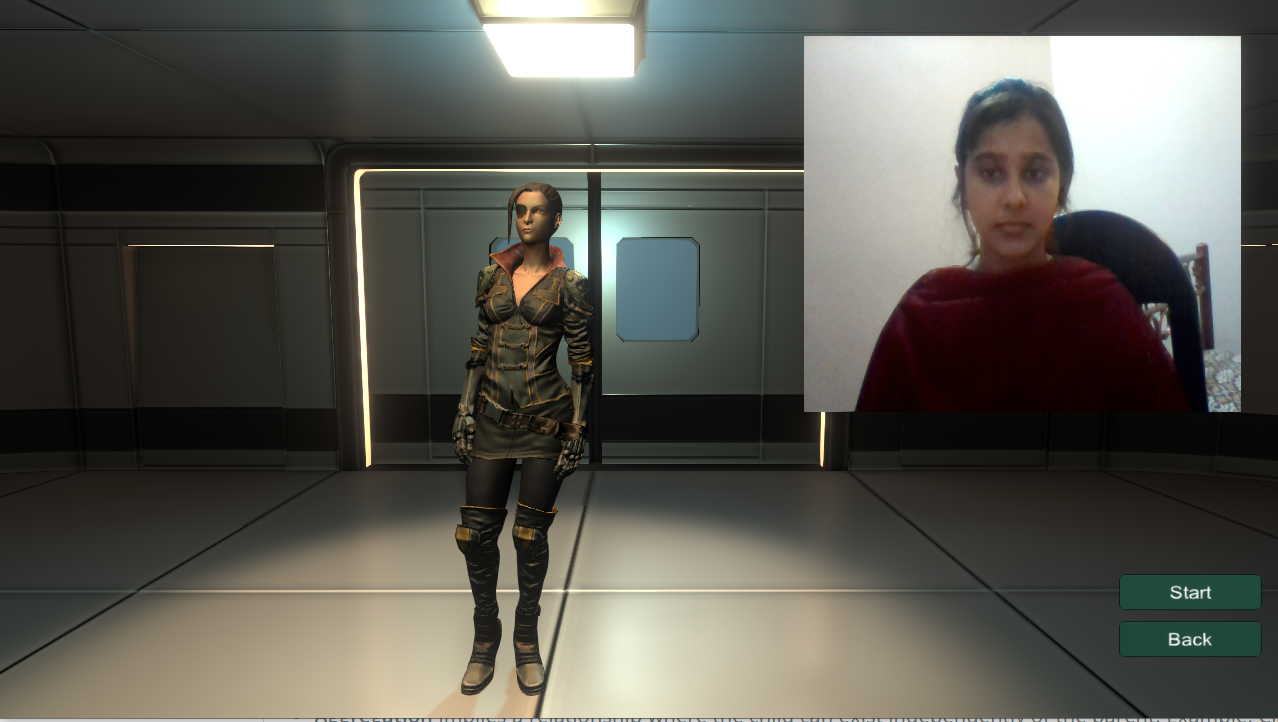
\includegraphics[scale=0.5]{images/screens/practice.png} 
  \caption{User Interface Practice and Fight Sessions} 
  \label{fig:practiceAndFightSessions}
\end{figure}

When the avatar animation has ended, unity communicates with the python script which then evaluates the user pose and gives feedback to the user. Figure \ref{fig:feedbackScreen} shows the feedback provided to the user after a practice session.

\begin{figure}
  \centering
  \subfigure[Feedback Provided to the User]{% 
    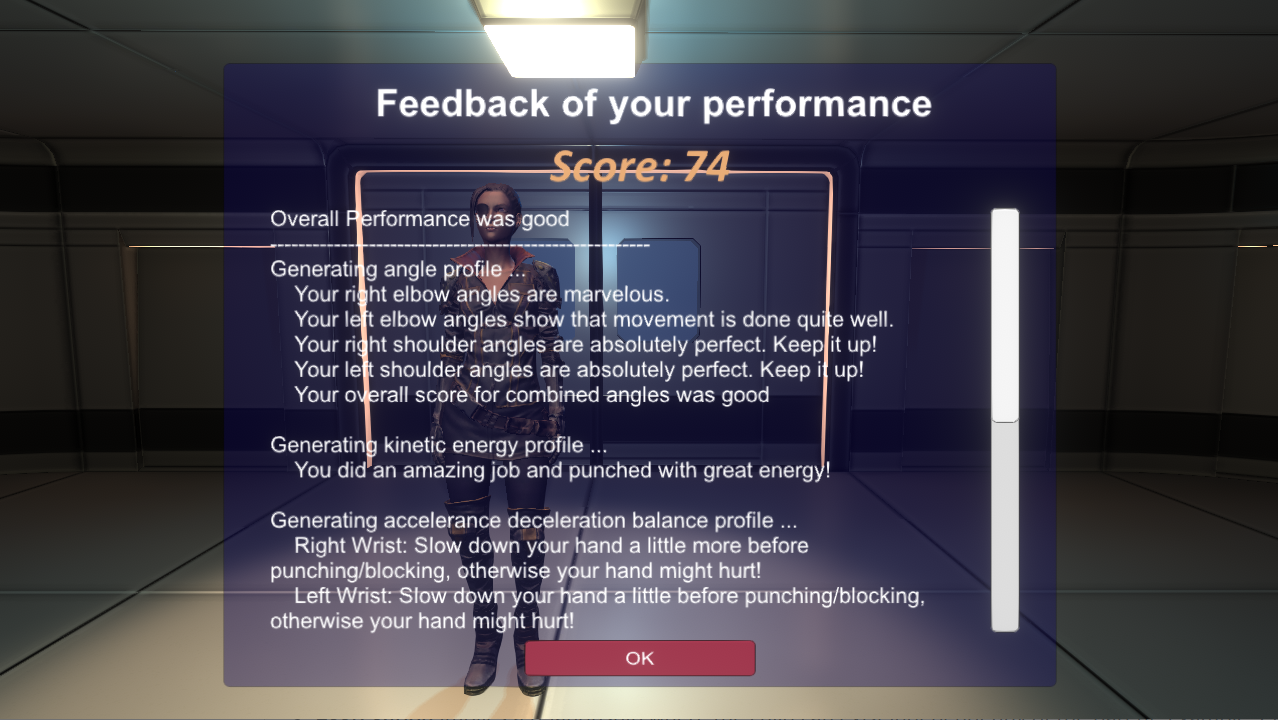
\includegraphics[scale=0.3]{images/screens/feedback1.png} \label{fig:feedback1} 
  } 
 \quad 
  \subfigure[Feedback Continued]{% 
   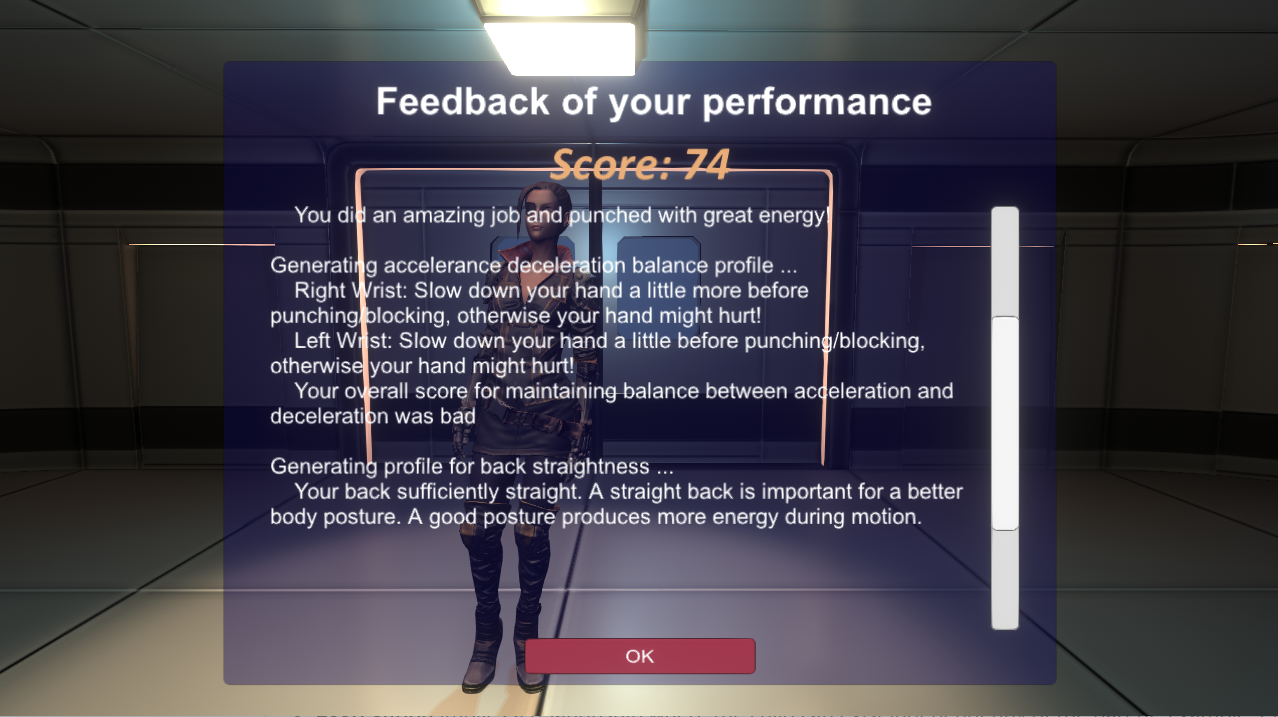
\includegraphics[scale=0.3]{images/screens/feedback2.png} 
   \label{fig:feedback2} 
  } 
  \caption{User Interface for Feedback Screen} 
  \label{fig:feedbackScreen}
\end{figure}


\section{Haptic Feedback Hardware Design}

The haptic feedback comprises of Electric muscle stimulation (EMS) source, the Transcutaneous electrical nerve stimulation (TENS) machine, and electrodes placed on the body. The hardware pipeline begins with an RGB camera capturing human images, during practice and fight sessions, at 30 fps and openpose producing the pose vector. To check if a user hits avatar, the wrist coordinate in the pose vector is checked if it collides with the avatar's bounding box. In case of a collision, a trigger is sent to an arduino system. This is the base of the hardware. This system activates the already calibrated TENS machine signals, at user specified spatial set of electrodes and amplitude level. In case of collision, it gives an impulse on the fist giving a sense of tap. It also locks the elbow by contracting the biceps/triceps. This contracting of muscles causes the arm to fold across the elbow joint. This gives an impression of arm being locked, since it is coupled with a person forcing a punch into the virtual avatar. Figure \ref{fig:punchSimulation} shows the placement of electrodes on arms and fists responsible for giving impulse on fists as an indication that some collision has occurred, and for locking the arm to prevent penetrating into the virtual objects. 

\begin{figure}
    \centering
    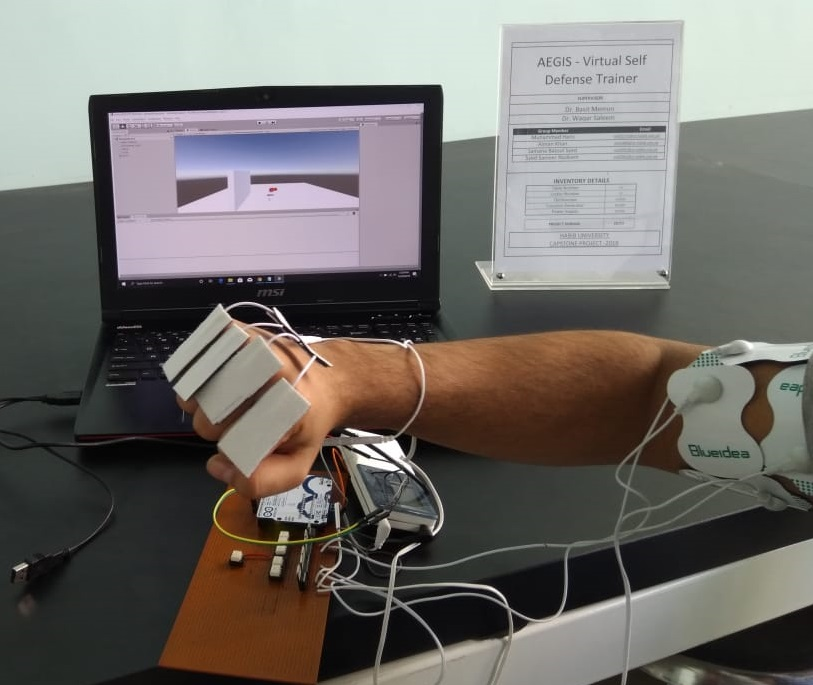
\includegraphics[scale=.7]{images/haptics/setup.jpg}
    \caption{Simulating a punch in the virtual world.}
    \label{fig:punchSimulation}
\end{figure}

The TENS machine we are using is the 'Digital TENS BE-660', a low frequency Digital TENS developed by Besmed. This device is connected with an Arduino Uno which communicates with unity through serial communication. The communication is one-way, that is, only Unity sends data to the arduino. The figure \ref{fig:besmed} shows the TENS machine and its components used.

\begin{figure}
    \centering
    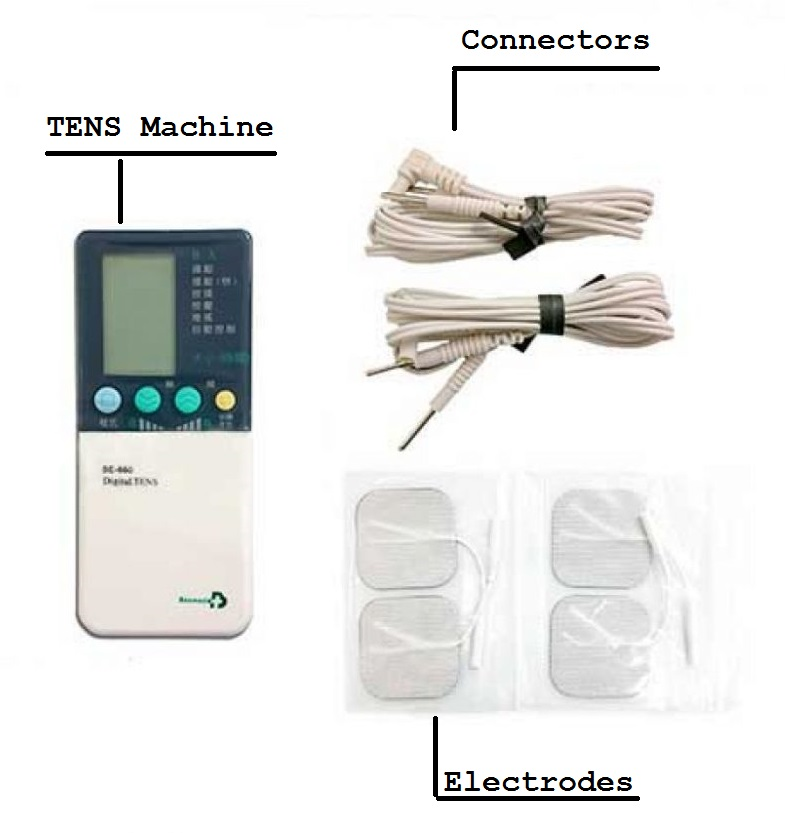
\includegraphics[scale=.5]{images/haptics/Besmed1.jpg}
    \caption{TENS Machine basic}
    \label{fig:besmed}
\end{figure}

In order to control the digital TENS with Arduino micro-controller the circuit, shown in figure \ref{fig:NodeCircuit}, is implemented on a PCB. The circuit works utilizing the principles of optotriacs. As the signal in query here is an AC signal generated by the TENs machine, normal switching to activate the haptics does not work. Therefore, a system of optocouplers and triacs is utilized. An Optocoupler is an electronic component that interconnects two separate electrical circuits using light-sensitive optical interface. Whenever needed, the arduino sends in a digital signal to the optocoupler to activate, which connects the circuit on the opposite end. For an AC signal, the optotriacs have a triac based opposite end, connecting the circuit, which further goes on to the primary triac connecting the electrode ends (one coming from the TENs and the other going to the muscles).

\begin{figure}
    \centering
    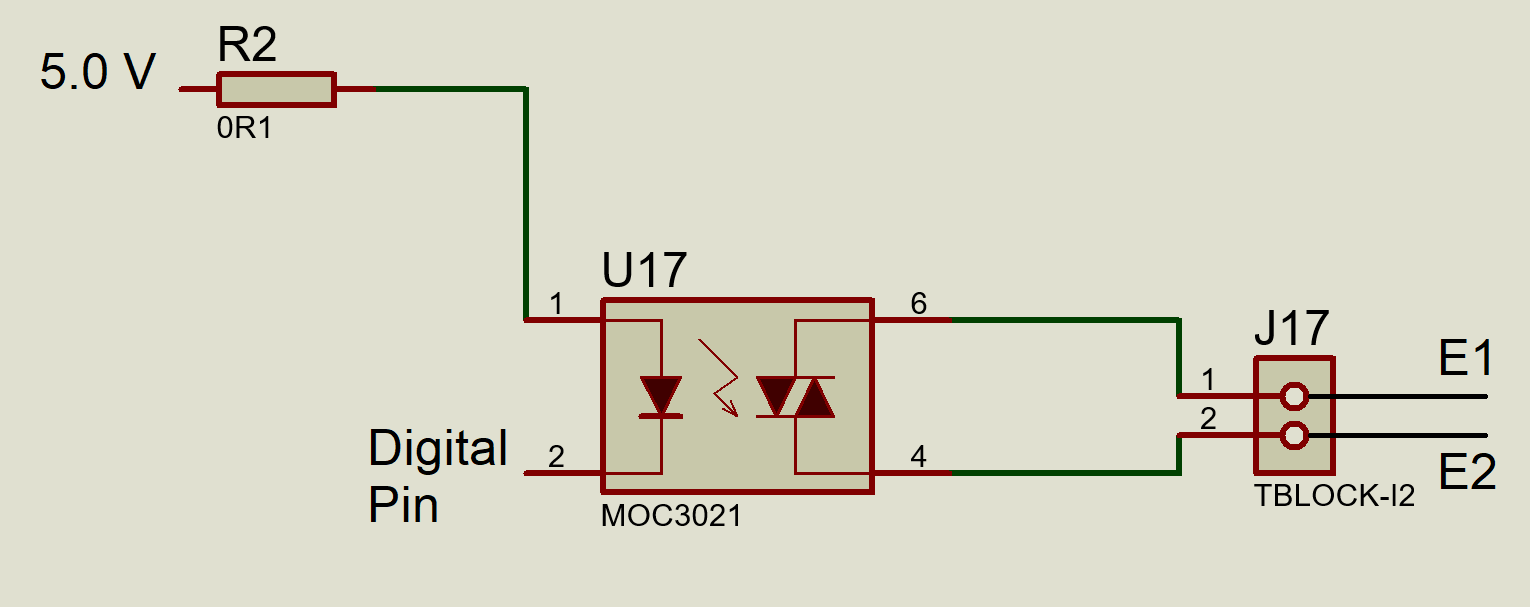
\includegraphics[scale=.5]{images/haptics/oneNodeCircuit.PNG}
    \caption{Single Node Circuit for Controlling TENS Machine via Arduino Microcontroller}
    \label{fig:NodeCircuit}
\end{figure}

A 3D model of the circuit implementation is shown in figure \ref{fig:circuit3d}

\begin{figure}
    \centering
    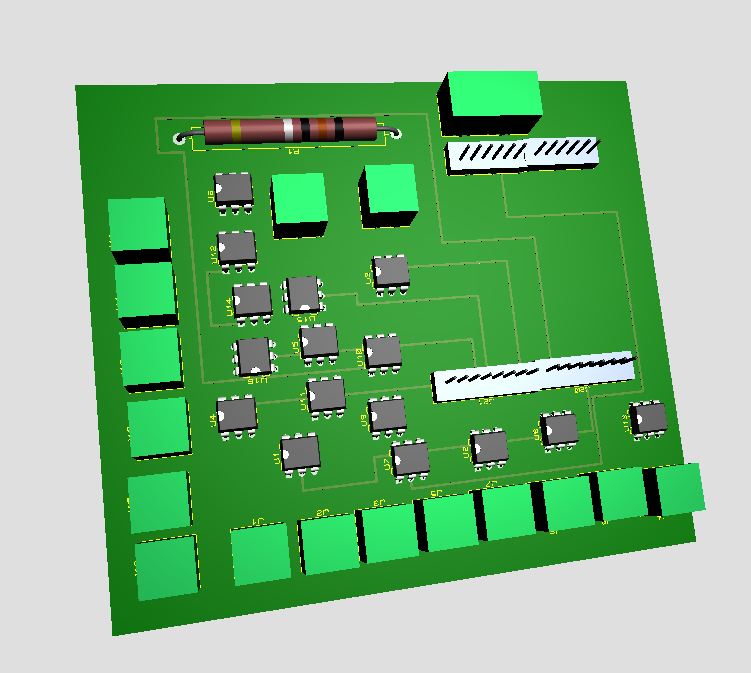
\includegraphics[scale=0.8]{images/haptics/circuit3D.PNG}
    \caption{3D Model of Circuit for Controlling TENS Machine via Arduino Microcontroller}
    \label{fig:circuit3d}
\end{figure}

The circuits in figures \ref{fig:NodeCircuit} and \ref{fig:circuit3d} have SIL (Single in Line) sockets for attaching Arduino UNO and T-Blocks for intercepting electrode wires. The Arduino UNO acts as an array of switches that short circuits electrode connections in a single T-block hence sending a signal to the body, when an appropriate collision trigger is sent from unity. 

The anatomical variations are the biggest limitation of designing a versatile haptic system using EMS. However, in order to overcome that hurdle, the system offers different spatial modes for electrodes, as shown in figure \ref{fig:spatialCal}, and intensity levels which are calibrated by user. Figure \ref{fig:hapticCallibration} shows the screen used for calibration. First a user needs to calibrate for impact feedback intensity and then for force feedback intensity followed by spatial location. The user will try out different combinations of intensities (and spatial setting in case of force feedback) and choose the one which does not hurt them but also feels realistic. 

Due to the pandemic the team was not able to test the haptic system robustly for a large number of people. It was however tested on a smaller set of people, which gave an affirmative response to the haptic feedback. 

\begin{figure}
    \centering
    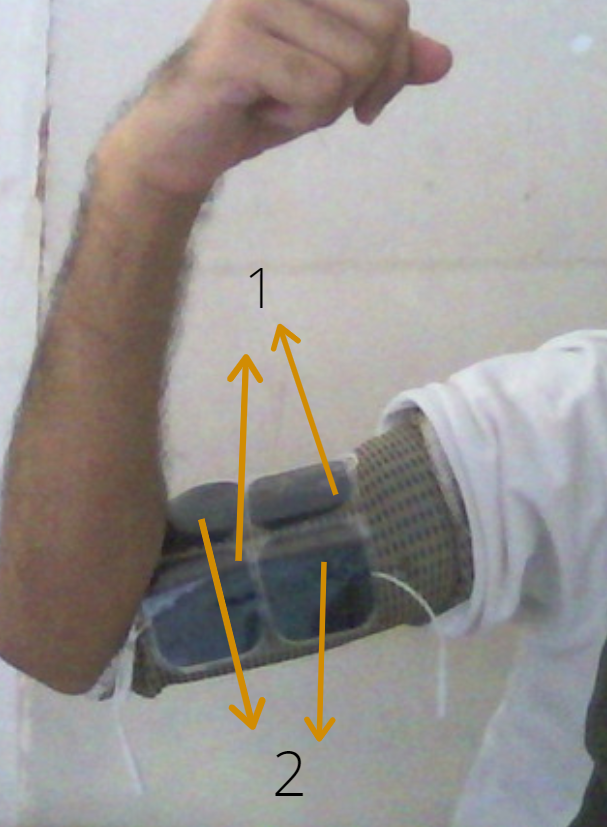
\includegraphics[scale=.5]{images/haptics/spatial.PNG}
    \caption{Spatial Calibration Modes for Electrodes}
    \label{fig:spatialCal}
\end{figure}

The haptic wearable, for both arms, is shown in figure \ref{fig:wearable}. This wearable entails impact feedback on hands for chop and punch, and forearms for blocking, and force feedback to cause the upper arm muscles to contract. This contraction prevents user from penetrating into virtual object and pushes the arm when the virtual object punches. For each signal to reach body 2 electrodes are required to complete the circuit. The materiel used for wearable is the surgical braces which is quite cheap and elastic. Hence they are comfortable to wear and fit almost all users. 

\begin{figure}
    \centering
    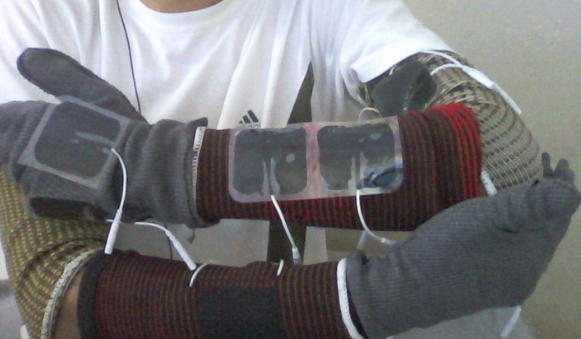
\includegraphics{images/haptics/wearable.PNG}
    \caption{Haptic Wearable}
    \label{fig:wearable}
\end{figure}

\section{Scoring Mechanism Pipeline}

As mentioned in the earlier sections system captures user's pose via a single RGB web camera and then computes a stick figure on each frame, via openpose, an returns a $18 \times 3$ matrix for each frame. Figure \ref{fig:stickFigure} shows stick figure of the human being superimposed on the original frame. These keypoints are compared with the keypoints obtained from the bench mark video sequence in order to compare the user movements. The scores assigned to user are relative to the benchmark performance. The procedure of assigning scores is not real time, the pose evaluation process runs after the user's performance has ended hence we do not need to output results in less than a second. 

\begin{figure}
    \centering
    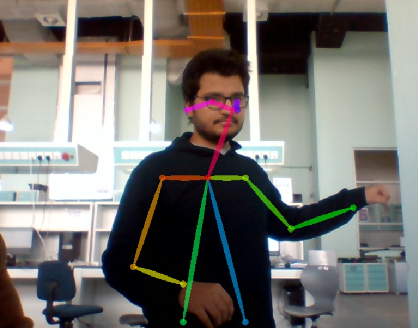
\includegraphics[scale=.75]{images/sketeton.png}
    \caption{Stick figure from openpose superimposed on original frame}
    \label{fig:stickFigure}
\end{figure}

Figure \ref{fig:scoringPipeline} shows the flow of scoring mechanism pipeline. Following are the different parts involved in pose evaluation.

\begin{figure}
  \centering
  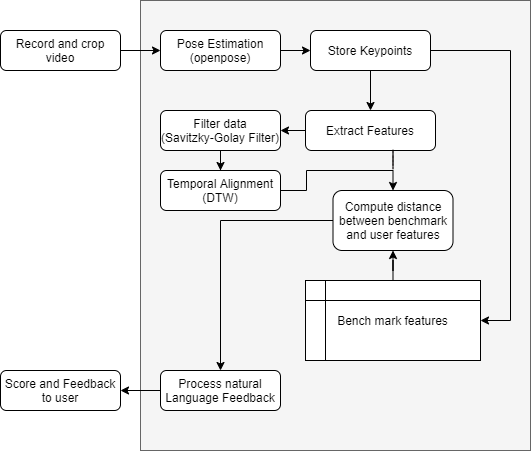
\includegraphics[scale=0.6]{images/scoringPipeline.png}
  \caption{Scoring Mechanism Pipeline Flow}
  \label{fig:scoringPipeline}
\end{figure}

\subsection{Pose Estimation}
When a practice or fight session ends, unity communicates with the python script responsible for estimating poses through openpose, on the images extracted through webcam during the session; %see Appendix \ref{appendix:code}. 
The pose estimation data is stored in a \texttt{.csv} file format that is used scoring mechanism for pose evaluation. 

\subsubsection{Openpose Parameters}
We have used "COCO" pose model that is trained on COCO dataset, and a net resolution of $-1 \times 80$ as the GPU machine did not allow for a net resolution greater than this due to insuffient memory, as described in section \ref{sub:designConstraints}. The number of maximum people that can be detected while pose estimation has been limited to just one, as we only need to detect one user only. The keypoint scaling has been set to 3 that normalizes all the estimated keypoints on a unit square from 0 to 1. 

\subsubsection{Writing Pose Data}

For each frame, 18 keypoints are extracted, and each keypoint is a 2D joint location along with the confidence score of that keypoint, hence each keypoint can be represented as \texttt{(x,y,CS)} where \texttt{CS} is the confidence score. The confidence scores are in the range [0,1]. Therefore, each frame data is represented as a $18 \times 3$ matrix. If openpose does not detect any human in a frame, then a $18 \times 3$ null matrix is pushed to the file. For $n$ frames, the \texttt{.csv} file contains $n \times 18$ rows of data. 

\subsubsection{Coordinate Transformation}
Openpose's coordinate system is different from python's coordinate system, hence all the keypoints are transformed to align with python's coordinate system so visualizing the data is clearer. 

\subsection{Feature Extraction and Scoring}

After pose estimation, the next task in the pipeline is to extract revelant features from  the data. Since we have only incorporated punch-block sequence in the project yet, the features are defined only for punch-block sequence. These features might change based on any other self-defense technique. For the punch-block sequence \cite{karatePunch} we have extracted the following features:

\begin{enumerate}
  \item Right shoulder and elbow angles 
  \item Left shoulder and elbow angles 
  \item Torso distance for calculating straightness of the back
  \item Kinetic energy 
  \item Acceleration and deceleration balance for biomechanical efficiency. 
\end{enumerate}

\subsubsection{Shoulder Angles}
Shoulder angles are calculated to make sure the user has performed the shoulder movements correctly. Correct shoulder movements are necessary for a proper punch. For example, if a user punches without displacing the elbow to the back first, then the punch looses most of its power and force. This displacing of elbow towards the back is captured by shoulder angle opening wide, and then shrinking again as the hand moves forward until it crosses the limbs, after which it starts to increase again. 

Shoulder angles are calculated through the equation \ref{eq:angle} where the middle joint becomes the origin, and $k_n, k_s$ and $k_e$ represents the neck, shoulder and elbow keypoints, and $J_{n,s}$ and $J_{e,s}$ represents the segments from neck  and elbow to shoulder respectively. 

\begin{gather}
  \textit{Neck to Shoulder Joint Segment}: J_{n,s} = K_n - K_s \\
  \textit{Shoulder Origin}: J_{s,s} = K_s - K_s = O \\
  \textit{Elbow to Shoulder Joint Segment}: J_{e,s} = K_e - K_s \\
  \alpha = cos^{-1} \big (\dfrac{J_{n,s} \cdot J_{e,s}}{||J_{n,s}|| ||J_{e,s}||})
  \label{eq:angle}
\end{gather}

These angles are computed for every frame, however the keypoint values are first filtered before extracting angles; section \ref{section:filteringSmoothing} talks more about filtering data. 

To calculate the score based on angles, we can not simply compare them with benchmark angles, as the probability that two users will produce perfectly aligned movements even if they are performing the exact same action, is extremely low. To solve this misalignment issue, dynamic time warping is used to temporally align the data of user and benchmark, this is described in detail in section \ref{section:dtw}

After dynamically warping the timed sequences of angles, the difference scores between both angle arrays are computed by calculating the absolute difference between them as shown in equation \ref{eq:angleDiffScore}. 
%However, the angle arrays are first multiplied by their confidence scores for each frame as shown in equation \ref{eq:angleTimesCS} where $A$ is the angle array and $CS$ is its confidence scores array, and the multiplication happens element-wise. The confidence score of an angle for frame $m$ contained by keypoints $K_{i,m}, K_{j,m}, K_{k,m}$ are calculated through equation \ref{eq:angleCS} where $CS_{i,m}, CS_{j,m}$ and $CS_{k,m}$ are confidence scores of keypoints $i,k$ and $k$ for frame $m$. 
These difference scores are then normalized to get on scale of 0-1 by dividing by the max difference score as shown in equation \ref{eq:normalizedAngleDiff}, and the similarity score is computed by subtracting 1 from it. 

%\begin{align}
  %\alpha_m = CS_{i,m} \cdot CS_{j,m} \cdot CS_{k,m}
  %\label{eq:angleCS}
%\end{align}
%\begin{align}
 % A_{CS} = A \cdot CS
  %\label{eq:angleTimesCS}
%\end{align}
\begin{align}
  \textit{Angle Difference Score:} \hspace{0.3cm} D_A = |A_{b} - A_{u}|
  %1 - \dfrac{A_{b,CS}  \cdot A_{u,CS}}{||A_{b,CS}|| \hspace{0.1cm} ||A_{u,CS}||}
  \label{eq:angleDiffScore}
\end{align}
\begin{align}
  D_A = \dfrac{D_A}{max(D_A)}
  \label{eq:normalizedAngleDiff}
\end{align}

\subsubsection{Elbow Angles}
Elbow angles are the key to effective blocking \cite{Karate}, and they also help in figuring out the characteristics of the punch,for example, elbow angles indicates the inclination of the forearm. If the forearm is flattened out towards the opponent just before hitting, it indicates a full punch, however, if the forearm is inclined at an angle, it means that the punch halted in the middle, and such a punch fails to deliver the entire force. 

Elbow angles are calculated just like shoulder angles, with shoulder, elbow and wrist keypoints. The elbow keypoint becomes the origin, the rest of the procedure is exactly similar as for the shoulder angles.

\subsubsection{Back Straightness}
The user should keep their back straight during any practice or fight session. A constant torso distance on average, which is the distance between the neck and the mid-hip keypoints, accounts for the straightness of the back \cite{movementQuality}. Back straightness is important because it makes the whole body aligned, producing significantly more power and gives a better balance \cite{movementQuality}. 

To calculate the torso distance, we need to calculate the distance between neck and the mid-hip keypoint for each frame. The mid-hip keypoint is calculated as the average of left and right hip keypoints. 

\begin{gather}
  \textit{Mid Hip} = \dfrac{\textit{Left Hip} + \textit{Right Hip}}{2}
  \label{eq:midhip}
\end{gather}

\begin{gather}
  Dist_t = \sqrt{\textit{Mid Hip Keypoint}^2 + \textit{Neck Keypoint}^2}
  \label{eq:torsoDistance}
\end{gather}

Because the torso length can change from one user to another, it is important to normalize the all the user's torso distance data by the maximum torso distance achieved in a specific frame \cite{movementQuality}. To compare this feature to the benchmark, an average value of torso distance is calculated which is used to estimate how much the average torso distance deviates from the benchmark. The score is computed by subtracting 1 from the difference score. 

\begin{gather}
  \overline{Dist_t} = \dfrac{ \sum_{i=1}^n \dfrac{Dist_t}{max(Dist_t)}}{n} \hspace{1cm} \textit{(n = number of frames)}
  \label{eq:avgTorsoDist}
\end{gather}

\begin{gather}
  Score_{BS} = 1 - \dfrac{|\overline{Dist_{b,t}} - \overline{Dist_{u,t}}|} { \overline{Dist_{b,t}}}
  \label{eq:torsoScore}
\end{gather}

If the user's average torso distance is lesser than the benchmark's average torso distance, it means that the user's posture of the back is incorrect. 

\subsubsection{Kinetic Energy}

The power with which an action is performed is one of the six good aspects of a good performance, according to the official guidelines for karate juries \cite{movementQuality}. The higher the velocity of the impact mass is, the more powerful (and consequently more efficient) the action is \cite{movementQuality}. As opposed to other researches which use kinetic energies extracted from all the keypoints, we use only 4 keypoints to extract kinetic energies: left wrist, right wrist, left elbow and right elbow. These 4 keypoints are selected because in a punch-block sequence, the most prominent velocity changes are happening in these 4 keypoints. The velocity of a keypoint is extracted using savitzky-golay filter. For each keypoint, the velocity values are calculated for each and every frame and the mass is inputed by the user through UI. 

For calculating an average score for kinetic energy, we calculated 2 scores and then the final kinetic energy score was computed as the average of these 2 scores, as shown in equation \ref{eq:overallKEScore}

For the first kinetic energy score, we were just interested in estimating the overall significant kinetic energy during the entire motion, we are not interested in individual kinetic energies of keypoints. Hence, we extract the kinetic energies of 4 keypoints, and then computed the average of these values to account for the overall significant kinetic energy during the performance, as shown in equation \ref{eq:kineticEnergy}, where $E_i$ refers to the kinetic energies of keypoint $i$, $n$ represents the number of frames, and $k$ is the total number of keypoints used for kinetic energy calculation. It was also normalized, so the score remains in the range [0,1].

\begin{gather}
  \overline{E} = \dfrac{\dfrac{\sum_{i=1}^k \sum_{j=1}^n E_i}{n * k}}{max(E)} 
  \label{eq:kineticEnergy}
\end{gather}

To compare this feature to the benchmark, a difference score is computed by estimating how much the average kinetic energy deviates from the respective benchmark feature. The score is computed by subtracting 1 from the difference score. However, if the user's kinetic energy is more than benchmark's kinetic energy, then the user is not penalized. 

\begin{gather}
  Score_{1,KE} = 
  \begin{cases}
    1 & E_b \leq E_u \\
    1 - \dfrac{|\overline{E_b} - \overline{E_u}|} { \overline{E_b}} & E_u < E_b \\
\end{cases}
  \label{eq:KEScore}
\end{gather}

The second difference score for kinetic energy was computed by taking the braycurtis distance between the kinetic energies of benchmark and user. The braycurtis distance between two vectors $u$ and $v$ is described in equation \ref{eq:braycurtis}:

\begin{align}
  d(u,v) = \dfrac{\sum_i (|u_i - v_i|)}{\sum_i (|u_i + v_i|)}
  \label{eq:braycurtis}
\end{align}

%\begin{align}
 % \textit{Kinetic Energy Difference Scores: } D_{KE} = \max_i |E_b - E_u|
%\end{align}

These difference scores are then normalized as shown in equation \ref{eq:KENormalized} so that they are in range [0,1]. The similarity score is computed by subtracting 1 from the difference score. 

\begin{align}
  D_{KE} = \dfrac{D_{KE} - min(D_{KE})}{max(D_{KE})-min(D_{KE})}
  \label{eq:KENormalized}
\end{align}

\begin{align}
  Score_{2,KE} = 1- D_{KE}
\end{align}

\begin{align}
  Score_{KE} = \dfrac{Score_{1,KE}+Score_{2,KE}}{2}
  \label{eq:overallKEScore}
\end{align}

\subsubsection{Biomechanical Effiency}
Biomechanical effiency of the motion refers to the balance between acceleration and deceleration. While punching, it is important that the user's acceleration of hand is balanced by its deceleration otherwise it might result in user hurting their hand \cite{movementQuality,scoringMultimodal}. The deceleration happens when at the end of an action, isometric muscles contract. 

To compute this balance, we need to compute the acceleration and deceleration time duration of both the wrist keypoints. The durations can not be calculated using acceleration and deceleration values hence we can not simply take the derivative of the velocity values. Therefore, to calculate the acceleration and deceleration time durations, we split the velocity time data into 2 phases using the maximum velocity of the motion \cite{scoringMultimodal}. In this way, the time duration before the maximum velocity is considered as acceleration phase, and the duration after maximum velocity is considered as deceleration phase, as shown in figure \ref{fig:accDectimes}.

\begin{figure}
    \centering
    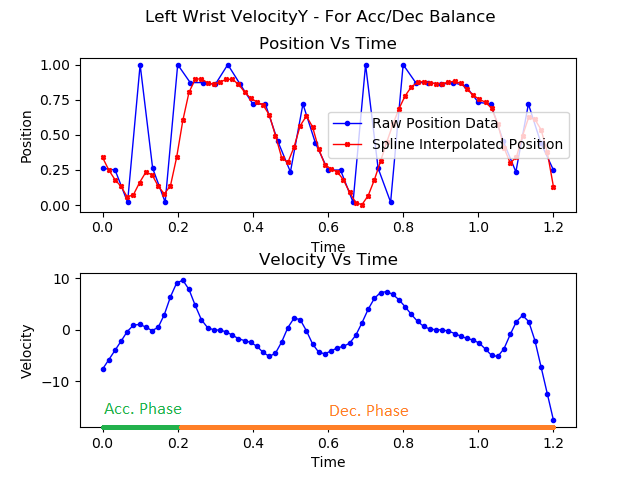
\includegraphics[scale=1]{images/graphs/accDecPhase_Video5_good_LWrist.png}
    \caption{Acceleration and deceleration phases in velocity time graph}
    \label{fig:accDectimes}
\end{figure}

Equation \ref{eq:balance1} shows how the balance between acceleration and deceleration is calculated. In an ideal case, where $t_{acc} == t_{dec}$, the balance is 1, i.e. maximum. 

\begin{gather} 
  B_1 = 1 - \dfrac{|t_{acc} - t_{dec}|}{t_{acc} + t_{dec}}
  \label{eq:balance1}
\end{gather}

However, some researches also suggests that there is no strict rule that the acceleration and deceleration duration should exactly be equal \cite{movementQuality}, it is possible that acceleration lasts for more time, hence a new balance score was computed where ideally acceleration time duration is expected to be 20\% more than the deceleration time duration, as described in equation \ref{eq:balance2}. Both these balance scores are then averaged to get a final balance score as shown in equation \ref{eq:balanceFinal}. 

\begin{gather} 
  B_2 = 1 - \dfrac{|t_{acc} - 1.2 \cdot t_{dec}|}{t_{acc} + 1.2 \cdot t_{dec}}
  \label{eq:balance2}
\end{gather}

\begin{gather} 
  B = \dfrac{B_1 + B_2}{2}
  \label{eq:balanceFinal}
\end{gather}

This balance score as described in equation \ref{eq:balanceFinal} can be used as a valid score, but to ease penalty on the user and to standardize every feature to be compared against its corresponding benchmark feature, it is further compared with the balance score of the benchmark to measure how much it deviates from the benchmark's balance score, as shown in equation \ref{eq:scoreBalance}. If the balance of user and benchmark is equal, then the balance similarity score will be 1, i.e. maximum.

\begin{gather} 
  Score_{B} = 1 - |B_u - B_b|
  \label{eq:scoreBalance}
\end{gather}

However, because the keypoints data is not stable, it is possible that the maximum velocity occurs right in the beginning or end of the motion, as shown in figure \ref{fig:accDectimes_maxAtStart}, which is wrong because every user starts motion with an idle position, and ends the motion with deceleration so it the maximum velocity can not occur at the very beginning or end of the motion.

To cater to this issue, we divide the velocity array into $k = 8$ sections, and discard the first and the last section while calculating max velocity. There is no restriction on the value of $k$, however, it should not be very small such that it discards large chunk of values, and should not be very big that it doesn't solve the problem stated. 

\begin{figure}
  \centering
  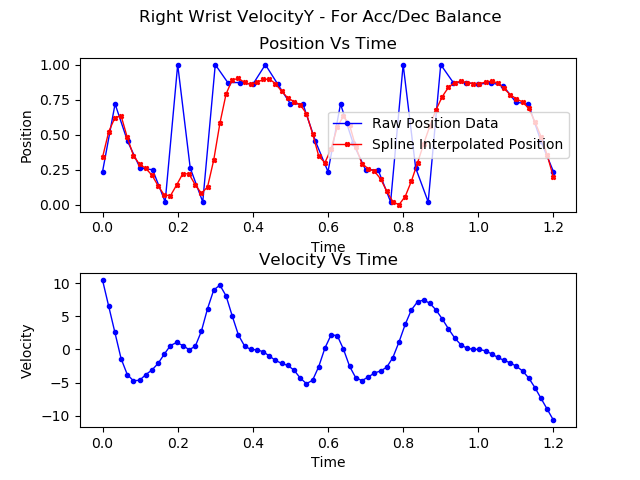
\includegraphics[scale=0.8]{images/graphs/accDecPhase_Video5_good_RWrist_MaxAtStart.png}
  \caption{Anomalies in velocity affecting balance between acceleration and deceleration}
  \label{fig:accDectimes_maxAtStart}
\end{figure}

The spline interpolation and velocity calculation in figures \ref{fig:accDectimes_maxAtStart} and \ref{fig:accDectimes} are further explained in section \ref{section:filteringSmoothing}

\subsection{Filtering and Smoothing Data}
\label{section:filteringSmoothing}
The common assumption made is that pose estimation is quite accurate however, this is not the case in our project. The raw keypoint data is very jerky and instable due to low net resolution inputted to openpose because of computer hardware constraints as described in section \ref{sub:designConstraints}. The raw data needs to be smoothened to be used further. 


Because of poor pose estimation, the extracted angles are cubic spline interpolated to give smooth results. This has helped improve the angle scores. Figure \ref{fig:anglesInterpolation} shows the differences in angle calculations with and without cubic spline interpolation. Figure \ref{fig:anglesWithoutInterpolation} shows discontinuities due to zero vector formed if any keypoint is not detected in a frame. This problem is removed automatically by interpolation. 

\begin{figure}
  \subfigure[Angles Without Interpolation]{% 
    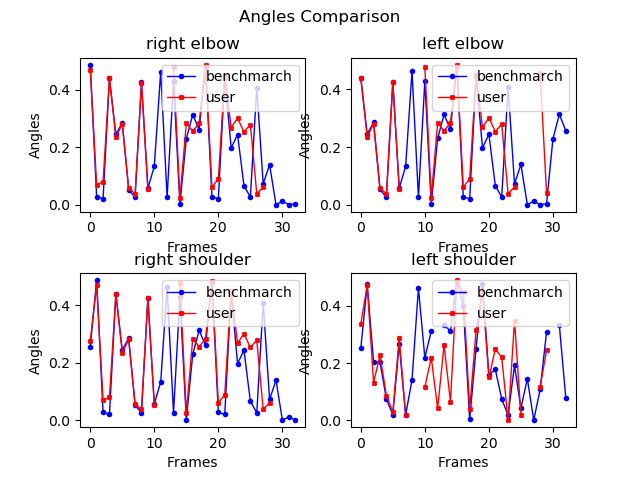
\includegraphics[scale=0.5]{images/graphs/anglesWithoutInterpolation.png} \label{fig:anglesWithoutInterpolation} 
  } 
 \quad 
  \subfigure[Angles With Interpolation]{% 
    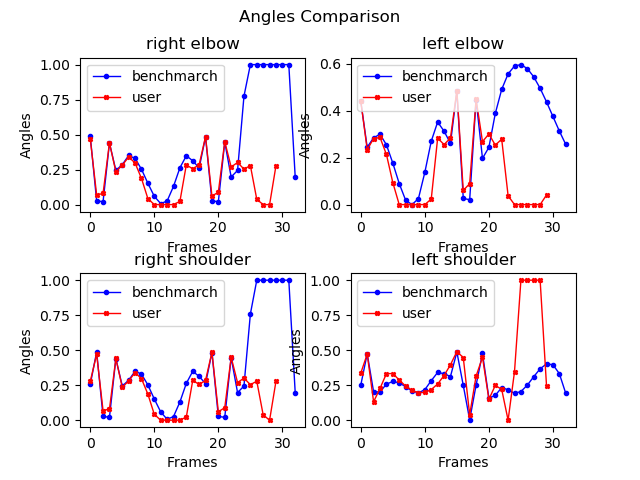
\includegraphics[scale=0.5]{images/graphs/anglesWithInterpolation.png} \label{fig:anglesWithInterpolation} 
  } 
  \caption{Differences in Angles With and Without Cubic Spline Interpolation} 
  \centering
  \label{fig:anglesInterpolation}
\end{figure}

Similarly, for velocity calculation, we can not directly take derivative of keypoint data because the data is very instable and jerky. For velocity calculation, we first ignore the keypoints location whose confidence score is below a minimum threshold, for example, in our case, for any keypoint $i$, we ignored its location from all the frames where its confidence score was below 0.2. The derivative is calculated through Savitzky-Golay filter, but after removing keypoint locations with confidence scores below the minimum threshold, the data becomes unequally spaced, and Savitzky-Golay filter can not be applied directly to this unequally spaced data. To solve this issue, the data is cubic spline interpolated. The cubic spline interpolation smoothes the keypoint data and also makes it equally spaced. 

Savitzky-Golay filter is a digital filter that can be applied to a set of digital data points for the purpose of smoothing the data, that is, to increase the precision of the data without distorting the signal tendency. For velocity calculation, a window size of 7 with order 2 (quadratic) is used to smoothen the data further and extract the derivative through this filter. The window size is selected in a way that the overall trend in the data is not lost and the spikes and jerks in data are removed, keeping nyquist criteria in view. 

Figure \ref{fig:velocitiesInterpolation} shows the differences in velocity calculations with and without cubic spline interpolation and confidence score filtering. Figure \ref{fig:velocitiesWithoutInterpolation} shows that if any keypoint is not detected during a frame, it distorts the entire velocity behavior and even changes the time at which the maximum velocity occurs. However, because with confidence score filtering, it already rejects the keypoints with low confidence scores, any keypoints which are not detected are automatically removed as they are predicted with a confidence score of zero. Therefore, the original behavior of the velocity is retained and further interpolation makes it smoother as shown in \ref{fig:velocitiesWithInterpolation}.

\begin{figure}
  \subfigure[Velocities Without Confidence Score Filter Interpolation]{% 
    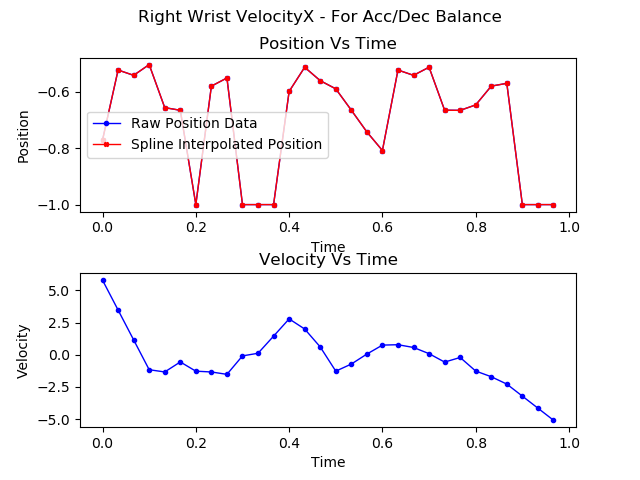
\includegraphics[scale=0.5]{images/graphs/velocitiesWithoutInterpolationAndFilter.png} \label{fig:velocitiesWithoutInterpolation} 
  } 
 \quad 
  \subfigure[Velocities With Confidence Score Filter and Interpolation]{% 
    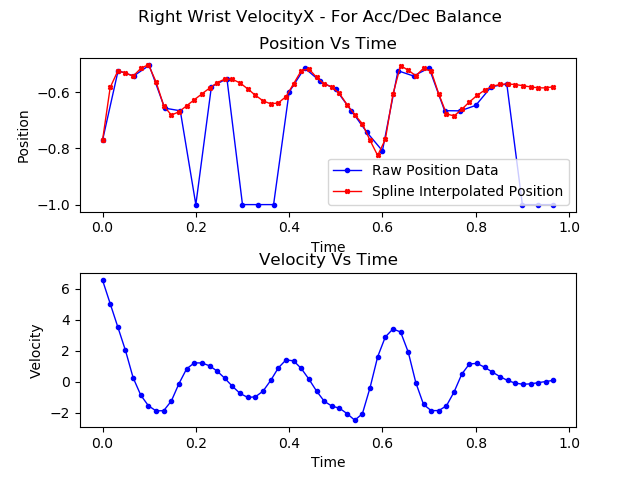
\includegraphics[scale=0.5]{images/graphs/velocitiesWithInterpolationAndFilter.png} \label{fig:velocitiesWithInterpolation} 
  } 
  \caption{Differences in Velocities With and Without Filtering and Cubic Spline Interpolation} 
  \centering
  \label{fig:velocitiesInterpolation}
\end{figure}


\subsection{Dynamic Time Warping}
\label{section:dtw}
To calculate the score based on angles, we can not simply compare them with benchmark angles, as the probability that two users will produce perfectly aligned movements even if they are performing the exact same action, is extremely low. So, even if a user has performed an action exactly like benchmark, it is highly unlikely that there will be frame to frame pose similarity because everyone performs at their own pace, some movements might be slower, some might be faster. Hence, it is impossible to compare frame to frame angles directly. To solve this misalignment issue, dynamic time warping is used to temporally align the frame data of user and benchmark.

For temporally aligning the frames of user and benchmark, a matrix is created which contains the distance (dissimilarity) of each frame of user against each frame of benchmark. For example, given $n$ frames from user's video, and $m$ frames from benchmark video, a dynamic time warping matrix (dtw matrix for short or $\mat D$) is created of order $m \times n$. Each matrix element is computed as the distance between vectors $m_i$ and $n_j$. These vectors are the flattened $18 \times 3$ matrices containing a frame's data. 

\subsubsection{Vector Dissimilarity Computation}
We implemented the following metrics to calculate the distance between each frame vector of benchmark $u$ and user $v$. 

\begin{enumerate}
  \item Cosine distance 
    \begin{align}
       d(u,v) = 1 - \dfrac{u \cdot v}{||u||_2  ||v||_2}
    \end{align}
  \item Correlation
    \begin{align}
      d(u,v) = 1 - \dfrac{(u- \overline{u}) \cdot (v- \overline{v})}{||(u- \overline{u})||_2  ||(v- \overline{v})||_2}
    \end{align}
  \item Euclidean distance
    \begin{align}
      d(u,v) = \sqrt{\sum_{i=1}^{n}(u_i - v_i)^2}
    \end{align}
  \item Absolute difference
    \begin{align}
      d(u,v) =  | u - v |
    \end{align}
\end{enumerate}

We noticed that normalizing the vectors $u$ and $v$ also impacts the distance between these vectors. However, none of these vector distance metrics were working either with or without normalization. This was happening because we were working with the entire frame data for each frame, and because except for a few keypoints, other keypoints either showed very minimal movements or were completely idle. This was making both the vectors $u$ and $v$ very similar and it has hard to compute the key difference between them which was essential for alignment. Hence, we introduced one more metric for computing distance between vectors $yu$ and $v$ which was to select only a subset of keypoints. 

\subsubsection{Optimal Path Calculation}

After creating the matrix, an optimal path from the matrix gives us the temporally aligned frames with maximum similarity. To find the optimal path, we start from matrix item $\mat D_{0,0}$ and move to the neighbour which has the minimum distance of all the immediate neighbours. The minimum distance ensures that we are selecting benchmark and user frame pair which the maximum similarity. Hence, the optimal path gives us the corresponding benchmark frames for each user frame, which had the maximum similarity with it and which also adheres to the temporal arrangement of the frames, i.e. if user frame $v_5$ is mapped to benchmark frame $u_{10}$, then user frame $v_4$ can never be mapped to any benchmark frame $u_i$ where $i > 10$. 

However, starting from $\mat D_{0,0}$ is a very strict requirement because it requires the first frames of both user and benchmark to be similar for the algorithm to work perfectly. For example, it is possible that the user starts the movement one fourth of a second later, in that case, the first frames of user and benchmark are not aligned, and thus the resulting optimal path won't be aligned too because at each step, the algorithm only sees its most immediate neighbours. Hence, the optimal path algorithm starts from any of the first 5 frames of either user or benchmark based on which has the most minimum distance that is maximum similarity. Then, it searches the immediate right, down, and diagonal neighbours and goes to the location where distance value is the minimum. This process repeats until either the rows or columns of the matrix are exhausted. 

From any matrix element $\mat D_{i,j}$, the optimal path algorithm for a single step is described by equation \ref{eq:dtwOptimalPath}.

\begin{align}
  i,j = argmin_{i,j}
  \begin{cases}
    \mat D_{i+1,j}  \\
    \mat D_{i,j+1}  \\
    \mat D_{i+1,j+1} \\
    \label{eq:dtwOptimalPath}
\end{cases}
\end{align}

Figure \ref{fig:dtw_matrix} shows the dynamic time warping matrix constructed, where the columns correspond to user frames and the rows correspond to the benchmark frames, and the optimal path (shown as red) that gives the temporally aligned frames with maximum similarity. 

\begin{figure}
  \centering
  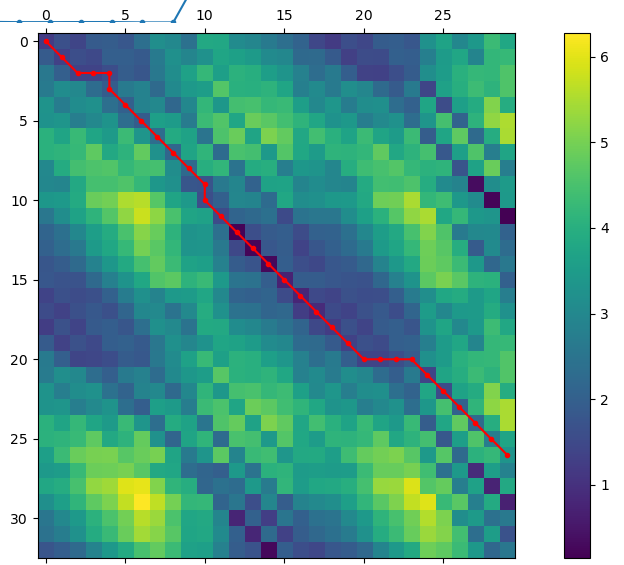
\includegraphics[scale=0.8]{images/graphs/dtw_matrix.png}
  \caption{Dynamic Time Warping Matrix and Optimal Path}
  \label{fig:dtw_matrix}
\end{figure}

\subsubsection{Metrics used in our software}
We found out that the temporal alignment works best on the following parameters.

\begin{enumerate}
  \item Metric = Absolute Difference,
  \item  Normalize = False,
  \item Selected 6 keypoints in frame data only, (right and left) shoulder, elbow and wrists keypoints.
\end{enumerate}

We found that the absolute difference metric outperforms all the other metrics implemented, and because differences are sensitive to magnitudes, not normalizing the vectors works better because they do not alter the magnitudes. Also, because during a punch, the significant movement only happens in these 6 keypoints mentioned above, we need to select only these, otherwise, because other keypoints either show very minimal movements or are completely idle, they average out the entire result and the key differences are lost which are essential for alignment.

\subsubsection{Results of Dynamic Time Warping}

Figure \ref{fig:originalAlignment} shows the original frame to frame alignment without using dynamic time warping for one specific instance in the entire performance. In this original alignment, the blocking action of the benchmark is incorrectly aligned with the punching action of the user. 
However, in figure \ref{fig:optimalAlignment}, which shows the optimal alignment between user and benchmark frame, the blocking action of the benchmark is correctly aligned with the blocking action of the user. 

\begin{figure} 
  \centering
  \subfigure[Benchmark Frame]{% 
    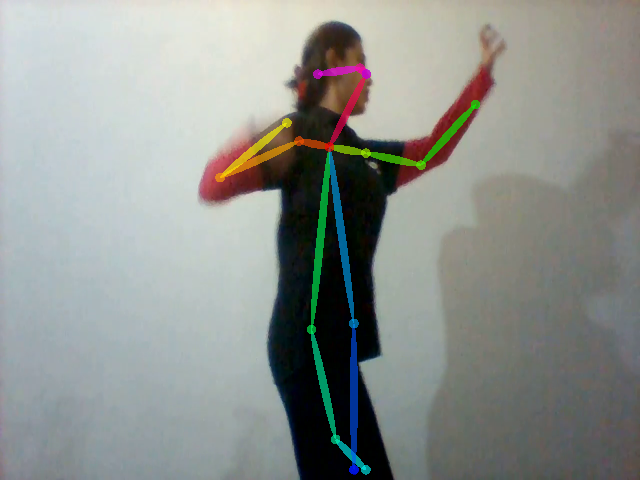
\includegraphics[scale=0.3]{images/dtw_alignment/benchmark_20.png} \label{fig:benchmarkFrame20} 
  } 
 \quad 
  \subfigure[User Frame]{% 
   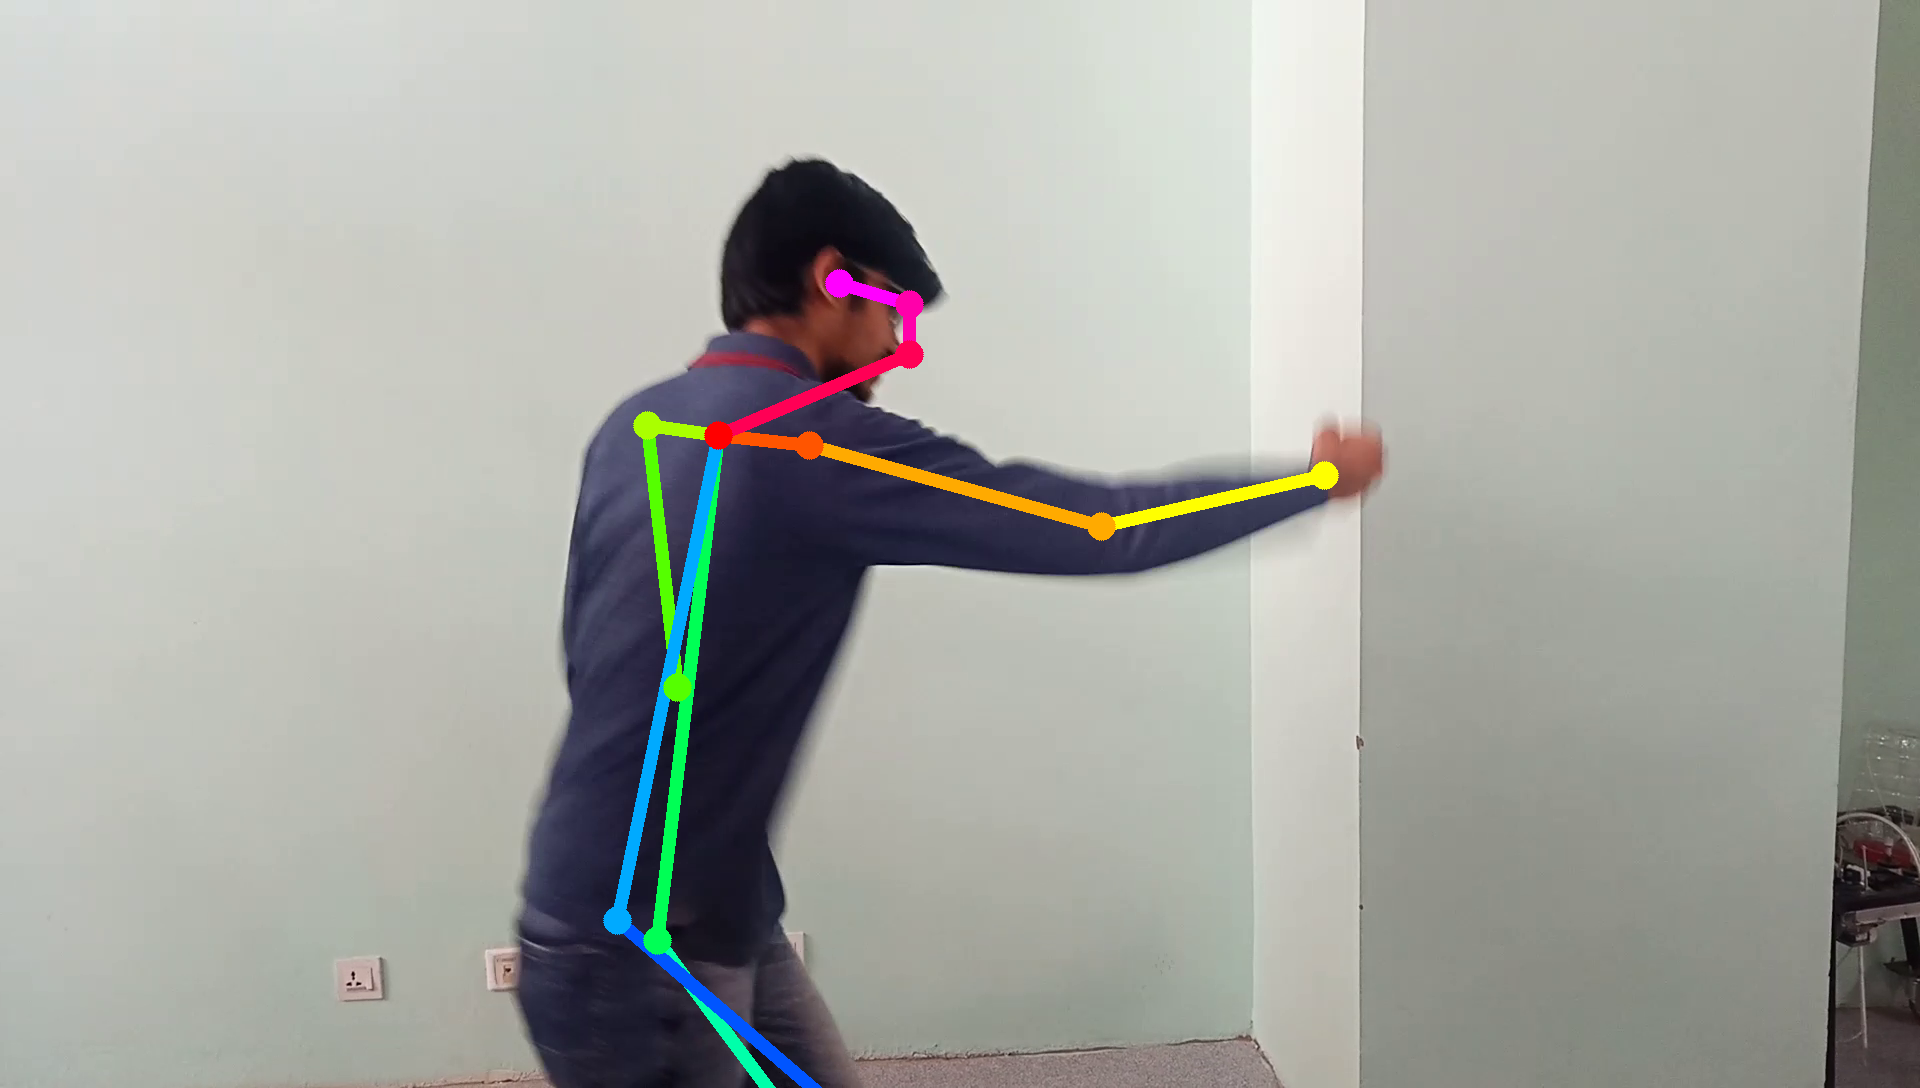
\includegraphics[scale=0.13]{images/dtw_alignment/user_20.png} 
   \label{fig:userFrame20} 
  } 
  \caption{Original Frame to Frame Mapping Without Dynamic Time Warping} 
  \label{fig:originalAlignment}
\end{figure}

\begin{figure} 
  \centering
  \subfigure[Benchmark Frame]{% 
    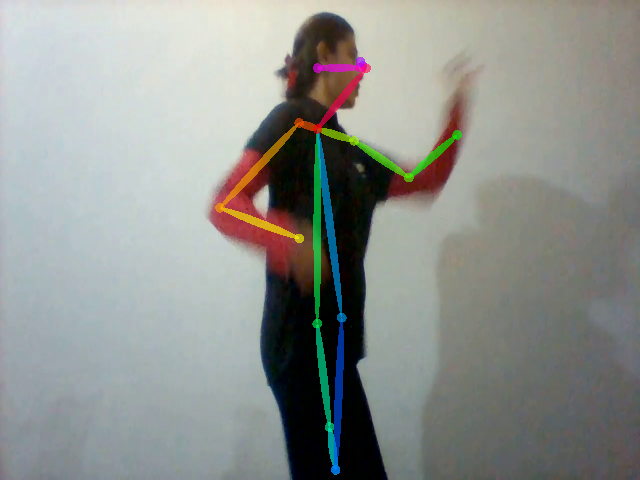
\includegraphics[scale=0.3]{images/dtw_alignment/benchmark_17.png} \label{fig:benchmarkFrame17} 
  } 
 \quad 
  \subfigure[User Frame]{% 
   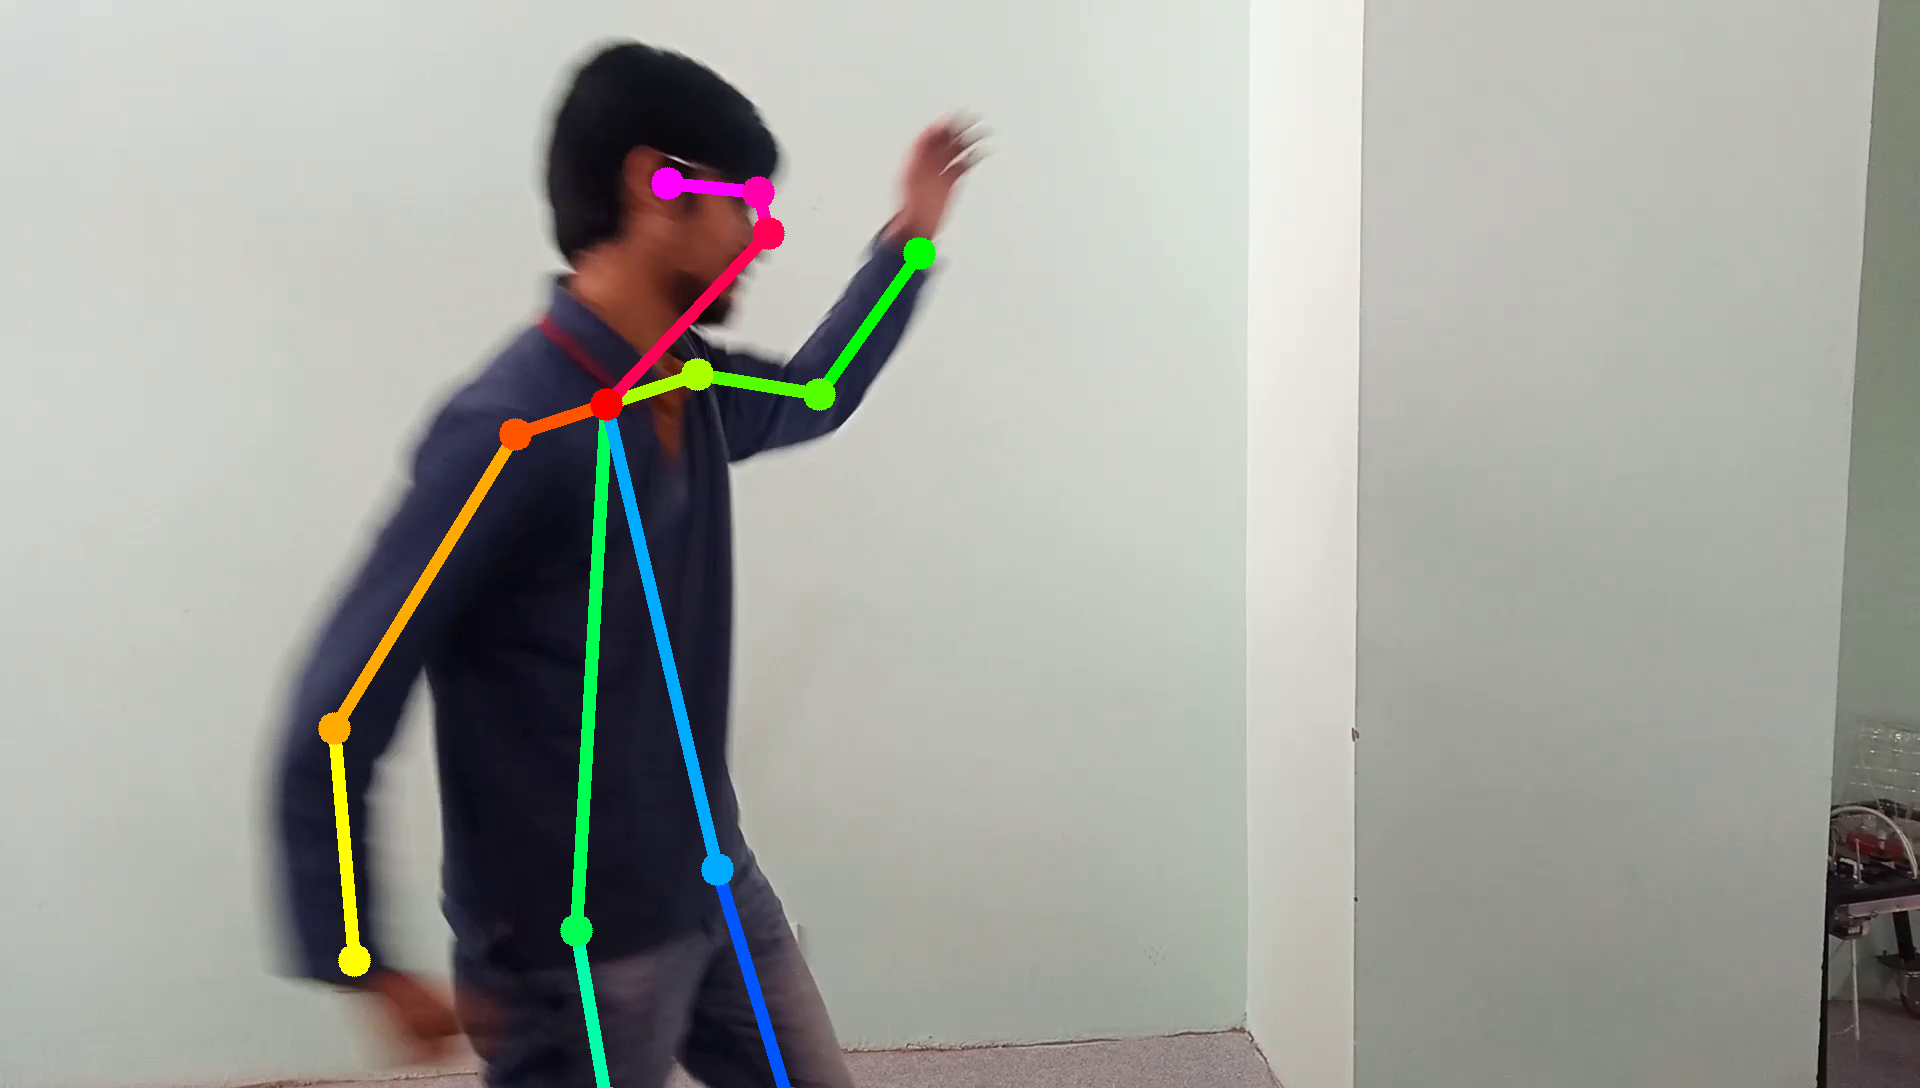
\includegraphics[scale=0.13]{images/dtw_alignment/user_12.png} 
   \label{fig:userFrame12} 
  } 
  \caption{Optimal Frame to Frame Mapping With Dynamic Time Warping} 
  \label{fig:optimalAlignment}
\end{figure}

\section{Feature-Based Classification and Feedback}
\label{section:classificationAndFeedback}

We classified each feature similarity score into categories good, average and bad. The classification was done through simple decision rules, as shown in equation \ref{eq:classification}.

\begin{align}
  \textit{Feature Category} = 
  \begin{cases}
    \textit{good} & \textit{Feature Score} > 78 \\
    \textit{bad} & \textit{Feature Score} < 55 \\
    \textit{average} & \textit{else}  \\
  \end{cases}
  \label{eq:classification}
\end{align}

These feature categories are used to generate feedback. From a phrases dictionary, the feedback for each feature is generated on the basis of its category, e.g. if angle features are categorized into 'good' category, then the phrases corresponding to good remarks about angles are outputted from the dictionary. Below is an example output for a bad performance:


\begin{lstlisting}
Generating angle profile ... 
	Your right elbow angles show that movement is done quite well.
	Your left elbow angles seem just fine.
	Your right shoulder angles show that movement is done quite well.
	Your left shoulder angles are okasish.
	Your overall score for combined angles was average

Generating kinetic energy profile ... 
	You were not able to produce enough energy during the motion. Try punching with more energy!

Generating accelerance deceleration balance profile ... 
	Right Wrist: Slow down your hand a little before punching/blocking, otherwise your hand might hurt!
	Left Wrist: Slow down your hand a little before punching/blocking, otherwise your hand might hurt!
	Your overall score for maintaining balance between acceleration and deceleration was bad

Generating profile for back straightness ... 
	Your back sufficiently straight. A straight back is important for a better body posture. A good posture produces more energy during motion.
\end{lstlisting}

The overall classification is also done on the basis of individual feature classification. Each feature contains a pre-defined weight. To classify the overall performance, it is categorized into its feature class according to its weight. For example, if there are 4 features $\{F_1, F_2, F_3,F_4\}$ with weights $\{0.3, 0.4, 0.15, 0.15\}$ and each feature is classified into $\{\textit{average}, \textit{good}, \textit{good},\textit{bad}\}$ respectively, then the performance category belongs to the category with the most weight, i.e. category good, as explained by equation \ref{eq:overallClassification}. 

\begin{align}
  \textit{Performance Category} = max
  \begin{cases}
    Weight: 0.4 + 0.15 & \textit{good} \\
    Weight: 0.3 & \textit{bad}  \\
    Weight: 0.15 & \textit{average} \\
  \end{cases} 
  \label{eq:overallClassification}
\end{align}




 


% TODO: Modify the chapter title appropriately your Kaaivsh.
\chapter{Implementation/Experiments and Results}
\label{chap:results}
\section{Pose Evaluation Results on Angles}

Angle Scores for video 4: 
  \begin{enumerate}
      \item 'right elbow': 0.8025153652097735, 
      \item 'left elbow': 0.7391806013546279, 
      \item 'right shoulder': 0.839144239263979, 
      \item 'left shoulder': 0.8246632634131507, 
      \item 'overall': 0.8013758673103827
  \end{enumerate}

  Angle Scores for video 6: 
  \begin{enumerate}
    \item 'right elbow': 0.9368570780248358, 
    \item 'left elbow': 0.7822153018489785, 
    \item 'right shoulder': 0.9357960950901351, 
    \item 'left shoulder': 0.7147700852047657, 
    \item 'overall': 0.8424096400421788
  \end{enumerate}

\begin{figure}[ht] 
    \subfigure[Angle Results on Video 4]{% 
      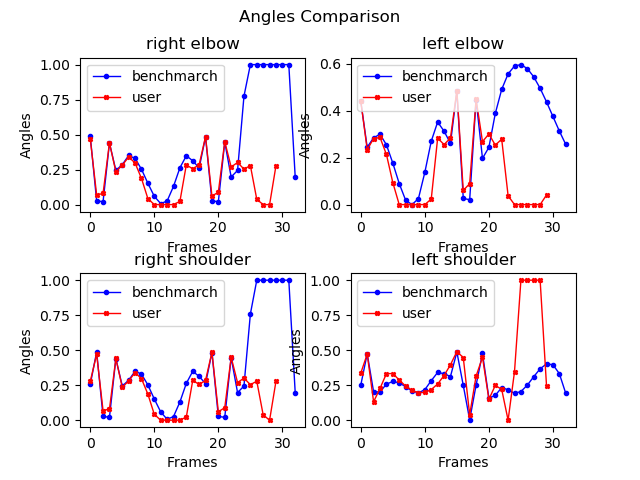
\includegraphics[scale=0.5]{images/graphs/angles_video4_good} \label{fig:video4_angles} 
    } 
   \quad 
    \subfigure[Angle Results on Video 6]{% 
      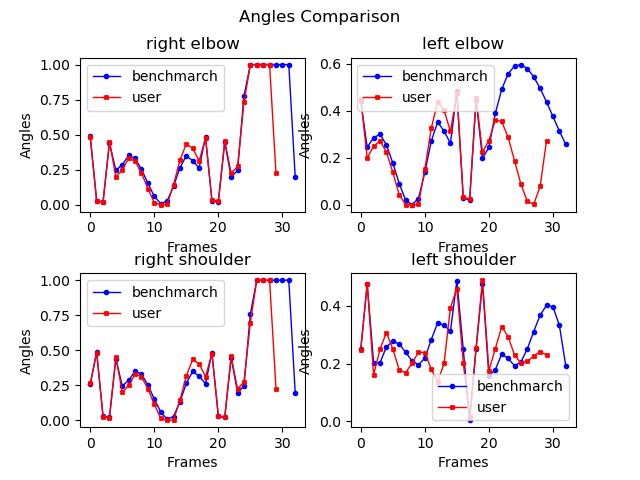
\includegraphics[scale=0.5]{images/graphs/angles_video6_good} \label{fig:video6_angles} 
    } 
    \caption{Angle Results on Good Videos} 
    \centering
    \label{fig:angles_good}
  \end{figure}

  Angle Scores for video 17: 
  \begin{enumerate}
      \item 'right elbow': 0.628917146659598, 
      \item 'left elbow': 0.6475396937624317, 
      \item 'right shoulder': 0.6398373397920147, 
      \item 'left shoulder': 0.6015687895010977, 
      \item 'overall': 0.6294657424287855
  \end{enumerate}

  Angle Scores for video 14: 
  \begin{enumerate}
      \item 'right elbow': 0.76486706531242, 
      \item 'left elbow': 0.46757149659087116, 
      \item 'right shoulder': 0.7364141153612161, 
      \item 'left shoulder': 0.5766052103240107, 
      \item 'overall': 0.6363644718971295
  \end{enumerate}

  \begin{figure}[ht] 
    \subfigure[Angle Results on Video 14]{% 
      \includegraphics[scale=0.5]{images/graphs/angles_video14_bad} \label{fig:video14_angles} 
    } 
   \quad 
    \subfigure[Angle Results on Video 17]{% 
      \includegraphics[scale=0.5]{images/graphs/angles_video17_bad} \label{fig:video17_angles} 
    } 
    \caption{Angle Results on Bad Videos Videos} 
    \centering
    \label{fig:angles_bad}
  \end{figure}

  \section{Pose Evaluation Results on Kinetic Energies}
  \begin{figure}[ht] 
    \subfigure[Kinetic Energy Results on Video 5 - Score: 83.5]{% 
      \includegraphics[scale=0.5]{images/graphs/KE_video5_good} \label{fig:video5_KE} 
    } 
   \quad 
    \subfigure[Kinetic Energy Results on Video 14 - Score: 62]{% 
      \includegraphics[scale=0.5]{images/graphs/KE_video14_bad} \label{fig:video14_KE} 
    } 
    \caption{Kinetic Energy Results} 
    \centering
    \label{fig:KE_results}
  \end{figure}

\section{Classification Results}
Following are the Classification Results:

\begin{lstlisting}[language=python, showstringspaces=false,frame=single]
    User Video: video1_good
    average
    ---------------------------------------------
    User Video: video2_good
    good
    ---------------------------------------------
    User Video: video3_good
    average
    ---------------------------------------------
    User Video: video4_good
    good
    ---------------------------------------------
    User Video: video5_good
    good
    ---------------------------------------------
    User Video: video6_good
    good
    ---------------------------------------------
    User Video: video8_average
    good
    ---------------------------------------------
    User Video: video9_average
    average
    ---------------------------------------------
    User Video: video10_average
    average
    ---------------------------------------------
    User Video: video11_average
    average
    ---------------------------------------------
    User Video: video12_average
    average
    ---------------------------------------------
    User Video: video13_average
    average
    ---------------------------------------------
    User Video: video14_bad
    average
    ---------------------------------------------
    User Video: video15_bad
    average
    ---------------------------------------------
    User Video: video16_bad
    average
    ---------------------------------------------
    User Video: video17_bad
    average
    ---------------------------------------------
    User Video: video18_bad
    good
    ---------------------------------------------
    
  
  \end{lstlisting}


\chapter{Conclusion and Future Work}
\label{chap:outro}
We have a working prototype of a virtual self defence training software offers video tutorials to users for learning punch-block sequence. It also provides practice sessions with a 3D virtual avatar, the sessions are integrated with pose evaluation module which is responsible for evaluating user's pose and provide feedback for improvement. In addition to detailed feedback, these sessions also provide realistic haptic feedback on the right during interaction with the avatar. We have been successful in amalgamating the positive aspects existing in literature including, but not limited to, natural language feedback, scoring user's performance, haptic calibration, force feedback and impact feedback using EMS and a user friendly user interface. 


Further work includes, extending the haptic feedback to both arms followed by fully body haptic suit and the use of EMG to replace manual calibration protocol. Other useful self-defense skills are yet to be incorporated into the system, so that it offers a complete set of basic self-defense skills to serve the purpose intended. The scoring mechanism can be further improved to incorporate more features. The practice sessions can be shifted to a virtual reality or augmented reality setting where the user interacts with the avatar that teaches directly, basically forming a dojo virtually. This technology can easily be applied to other training as well. Another important avenue to look at is the shifting of the computation, including and not limited to the pose evaluation to a cloud server so that the program can also be used by users having devices with lesser computation power as required. We can also get a self-defense trainer on board to rank and judge the feedback and scoring suggested by the system so we have a ground truth to work with and compare our system against, which could very likely improve the pose evaluation module. With huge number of dataset, we can also incorporate deep learning models that learn the features directly without identifying, because identifying the features takes a lot of work and study into the performance of a practicular skill. The possibilities to go further with this are limitless.


\appendix

% This appendix is optional.
\chapter{More Math}
Here, we describe the background math for the techniques used in the text.

% This appendix is required if the data set is not fully described in the main text.
\chapter{Data}
Here is a dump of our 2TB data set. Enjoy!

% This appendix is required if the code is not fully described in the main text.
\chapter{Code}
Here is our code. Bits over trees, courtesy of HEC!

% inspired by https://xkcd.com/221/
\begin{lstlisting}[language=python, showstringspaces=false,frame=single]
  print('Hello World!')
  print('Computing true random number.')
  print('Capturing interstellar radiation.')
  print('This will take time!')
  import random
  import time
  time.sleep(3600*random.randint(1,10))
  print(4)
\end{lstlisting}

% Alternately...
Our code can be found at \href{https://github.com/habib-university/Kaavish-Template}{this GitHub link}.

%%% Local Variables:
%%% mode: latex
%%% TeX-master: "../report"
%%% End:



% Print the bibliography with a ToC entry and titled, "Referneces".
\printbibliography[heading=bibintoc,title={References}]

\end{document}
